
\subsection{Studies in the General Phase Space} % (fold)
\label{sub:coarse_studies}

In order to examine the overall discrimination performance of the DNN's to that of the physics-driven variables, we examine the ROC curves in Figure~\ref{fig:combinedROC1}. In particular, we compare the DNN's to $n$-subjettiness~\cite{nsub} $\tau_{21} = \tau_{2}/\tau_{1}$, the jet mass, and the distance $\Delta R$ between the leading two $p_{T}$ subjets.  In Figure~\ref{fig:combinedROC1a}, we can see that the three DNN's have similar performance, but the MaxOut networks tends to outperform the ConvNet networks.  We suspect that the MaxOut tends to outperform the ConvNets due to sparsity of the jet-images, whereby the MaxOut network views the full jet-image from the inital hidden layer while the sparsity tends to make it difficult for the ConvNets to learn meaningful convolution filters .  We also see that the ConvNet-Norm tends to outperform the ConvNet trained on the un-normalized jet-images.  As we will see soon,  it is difficult for these networks to fully learn the jet mass and thus the loss of mass information from normalization and energy  binning (rather than transverse energy) of the ConvNet-Norm training tends to not to impede performance.   Finally, we can see the Fisher-Jet discriminant\footnote{The Fisher discriminant is trained in three partitions of $\Delta  R$ ($\Delta R \in [0.25, 0.5],\ [0.5, 0.75],\ [>0.75])$, in order to account for the non-linear variation in jet-images from the differing positions of the two subjets.  Also note that unlike in the original implementation, here we do not normalize the jet images when computing the Fisher Jet.  This leads to slightly better performance.} performance, as described in reference~\cite{Cogan:2014oua}, which outperforms the physics inspired variables (as expected) but is much less performant than the DNN's. In addition, in Figure~\ref{fig:combinedROC1b} we see that the DNN's also outperform the two-variable combinations of the physics inspired variables (computed using the 2D likelihood ratio).   It is interesting to note that combining mass and $\tau_{21}$, or $\tau_{21}$ and $\Delta R$, achieve much higher performance than the individual variables and are significantly closer to the performance of the DNN's.  However, the large difference in performance between the DNN's and the physics-variable combinations implies the DNN's may be learning information that is not \emph{fully} encapsulated in these physics variables.
%This is likely due to the normalization and energy binning helping to provide more uniformity in the typical pixel intensities across jet-images.
\begin{figure}[!htbp]
\begin{center}
\subfloat[]{
	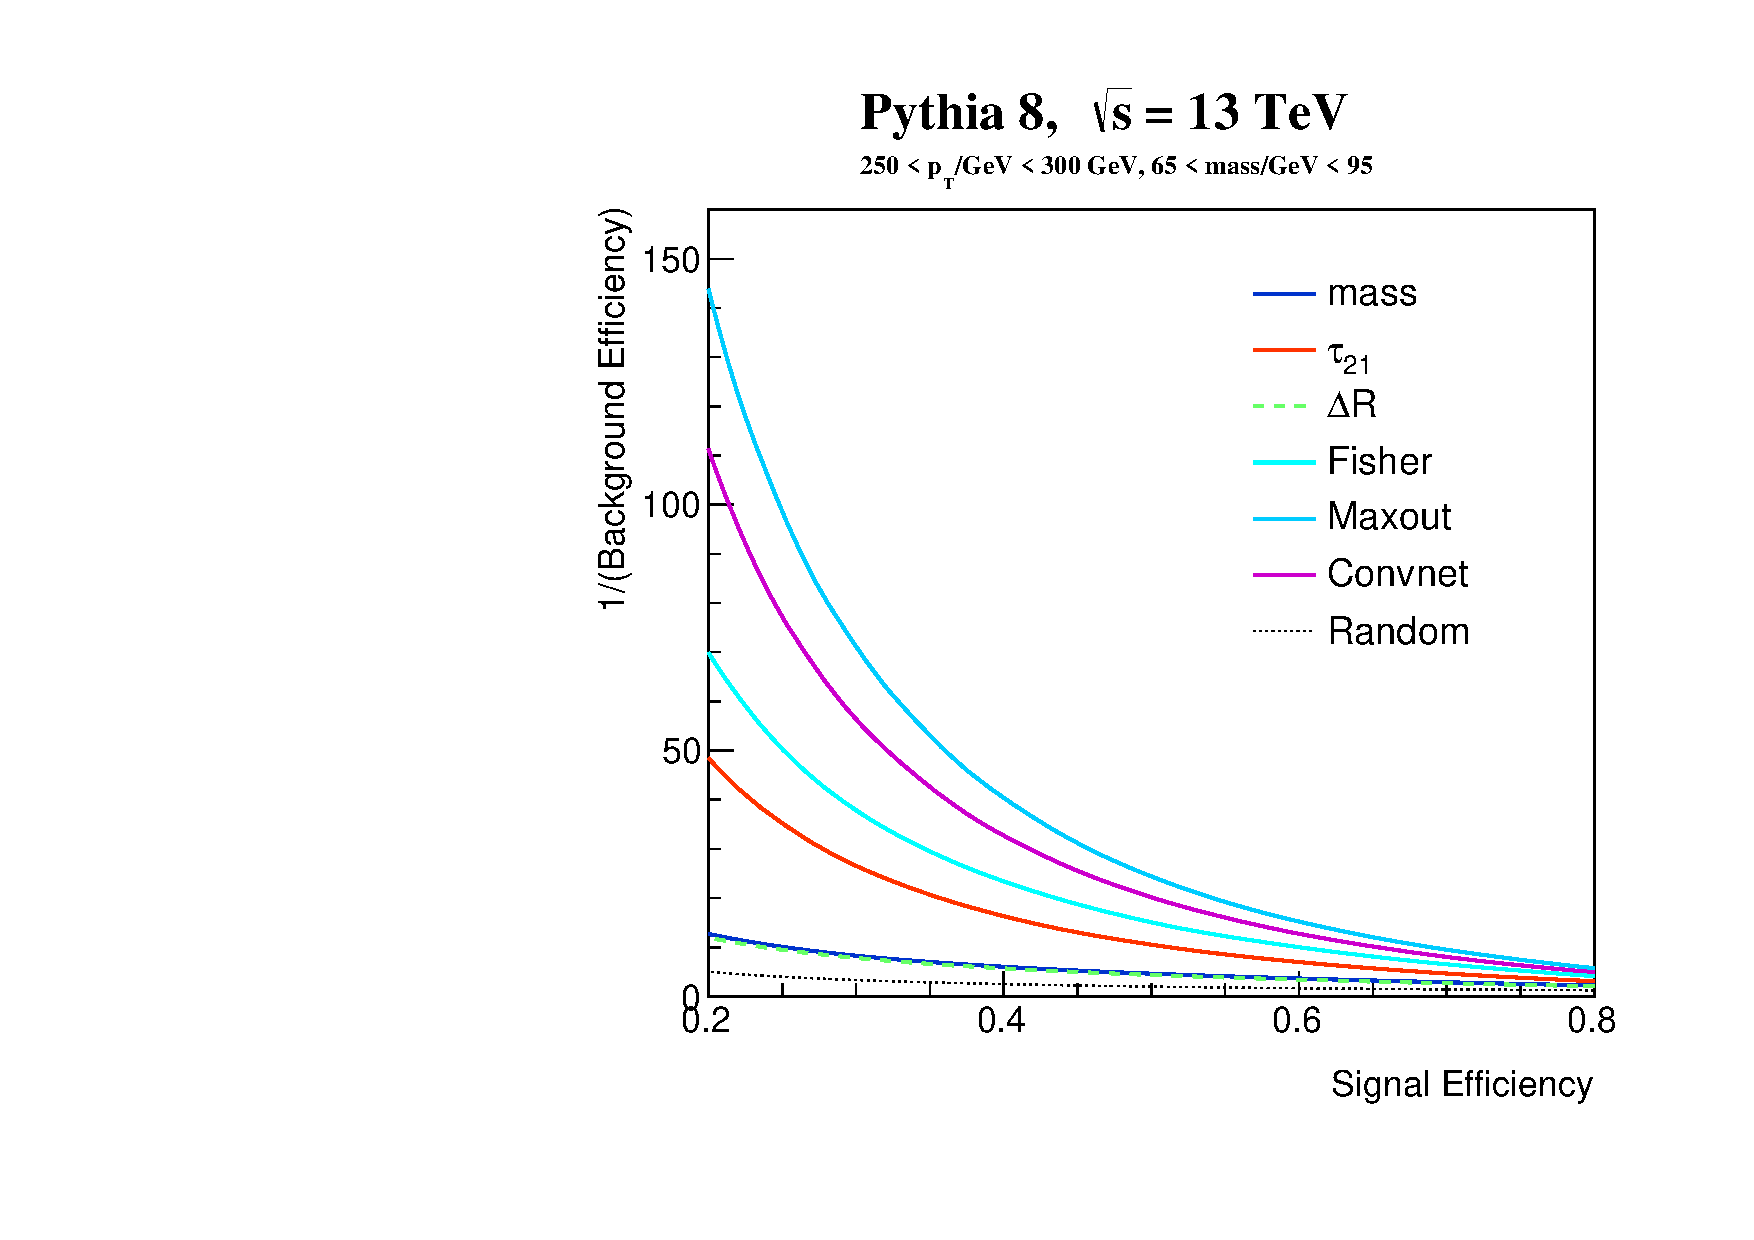
\includegraphics[width=0.48\textwidth,angle=0]{figures/ROC_1}
	\label{fig:combinedROC1a}
}
\subfloat[]{
	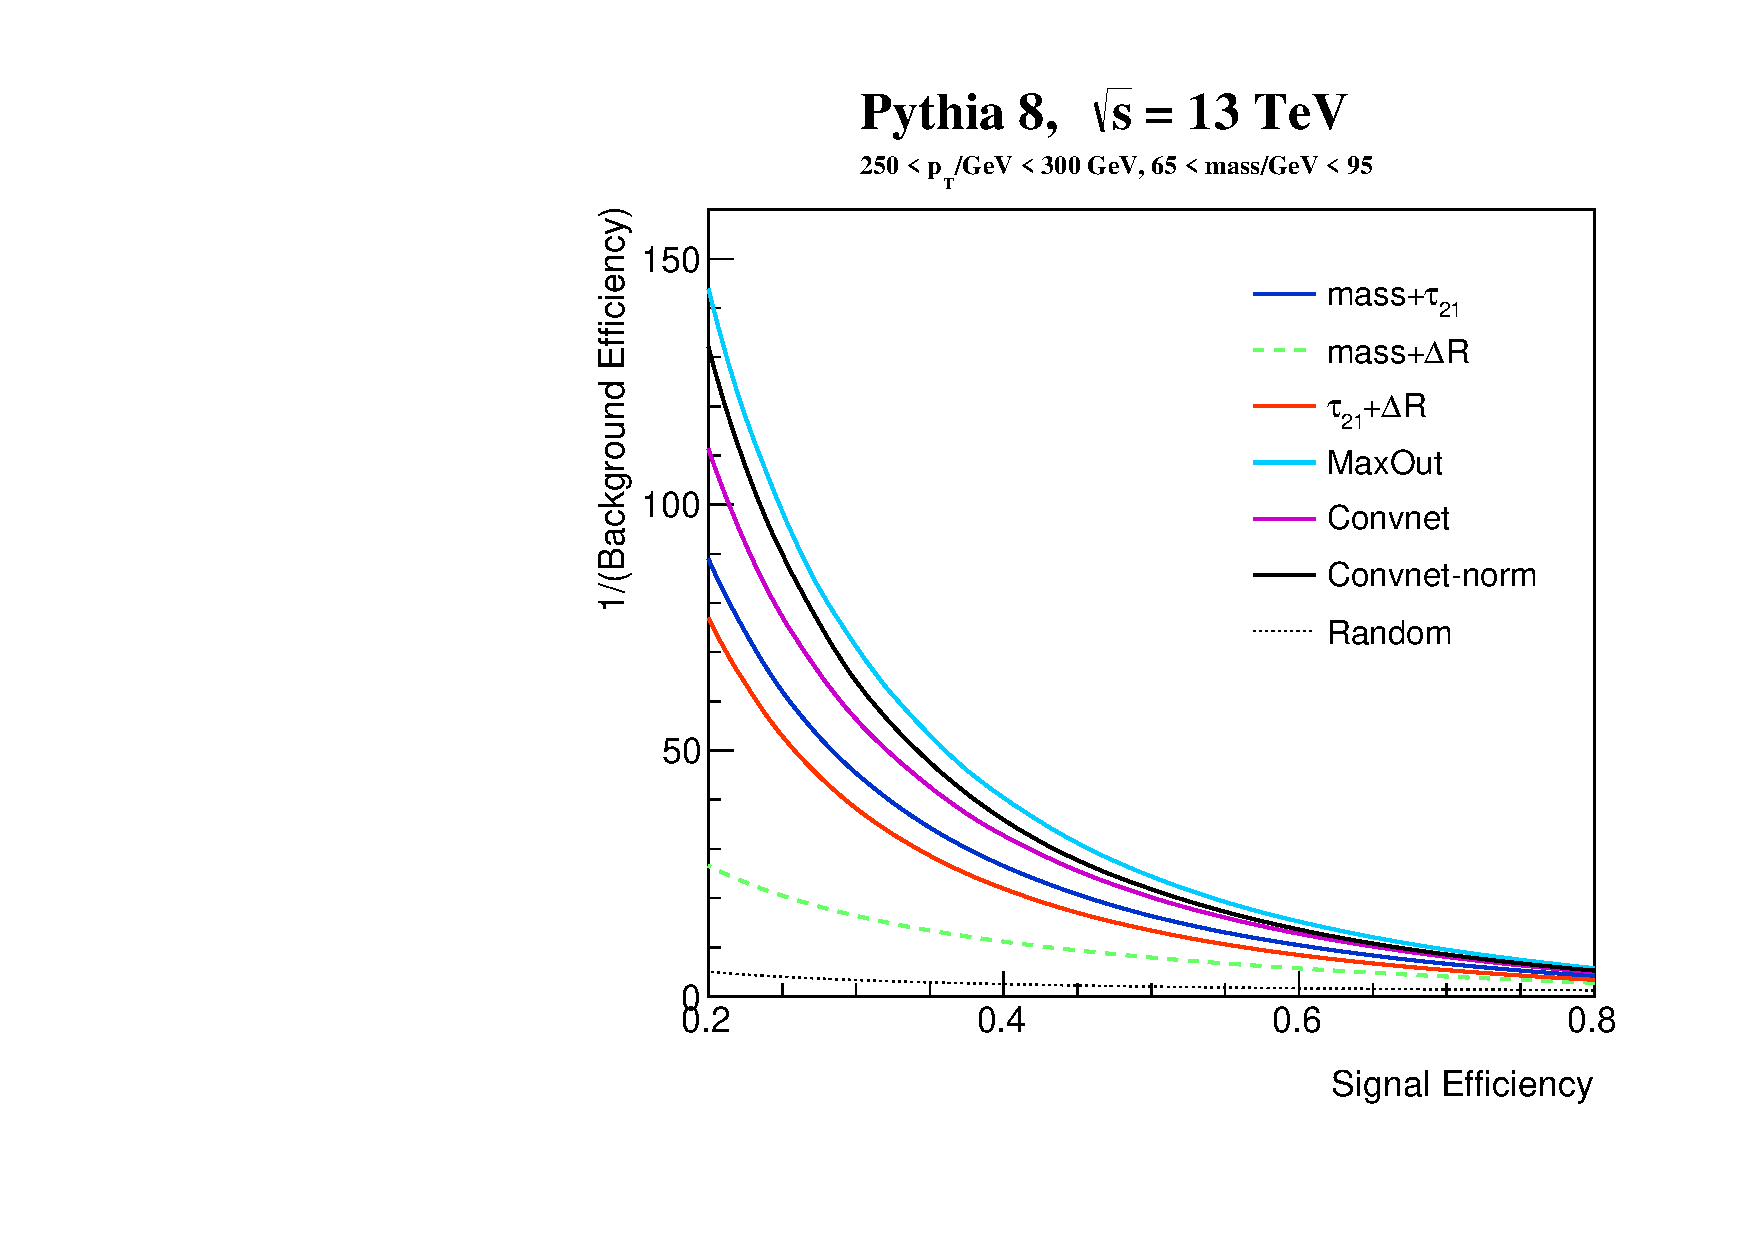
\includegraphics[width=0.48\textwidth,angle=0]{figures/ROC_2}
	\label{fig:combinedROC1b}
}
\end{center}
   \caption{Receiver Operating Characteristic (ROC) over coarse sample}
  \label{fig:combinedROC1}
\end{figure}


While we can see in Figure~\ref{fig:combinedROC1} that the DNN's outperform the individual and two-variable physics inspired discriminators, we want to understand if these physics variables have been learned by the networks.  As such, we compute the combination of the DNN's with each of the physics inspired variables (using the 2D likelihood), as seen for the ConvNet in Figure~\ref{fig:combinedROC2a} and for the MaxOut network in Figure~\ref{fig:combinedROC2b}. In both cases, we see that the discriminators combining $\Delta R$ or $\tau_{21}$ with the DNN's does not improve performance.  This indicate that the information contained in these physics-inspired variables  has already been fully learned by the networks.  However, adding mass in combination with the DNN's shows a noticeable improvement in performance over the DNN's alone.  This indicates that all of the information contained in the mass variable has not been learned by the DNN's.  While it is not shown, similar patterns are found for the Conv-Norm network.
\begin{figure}[!htbp]
  \begin{center}
\subfloat[]{
	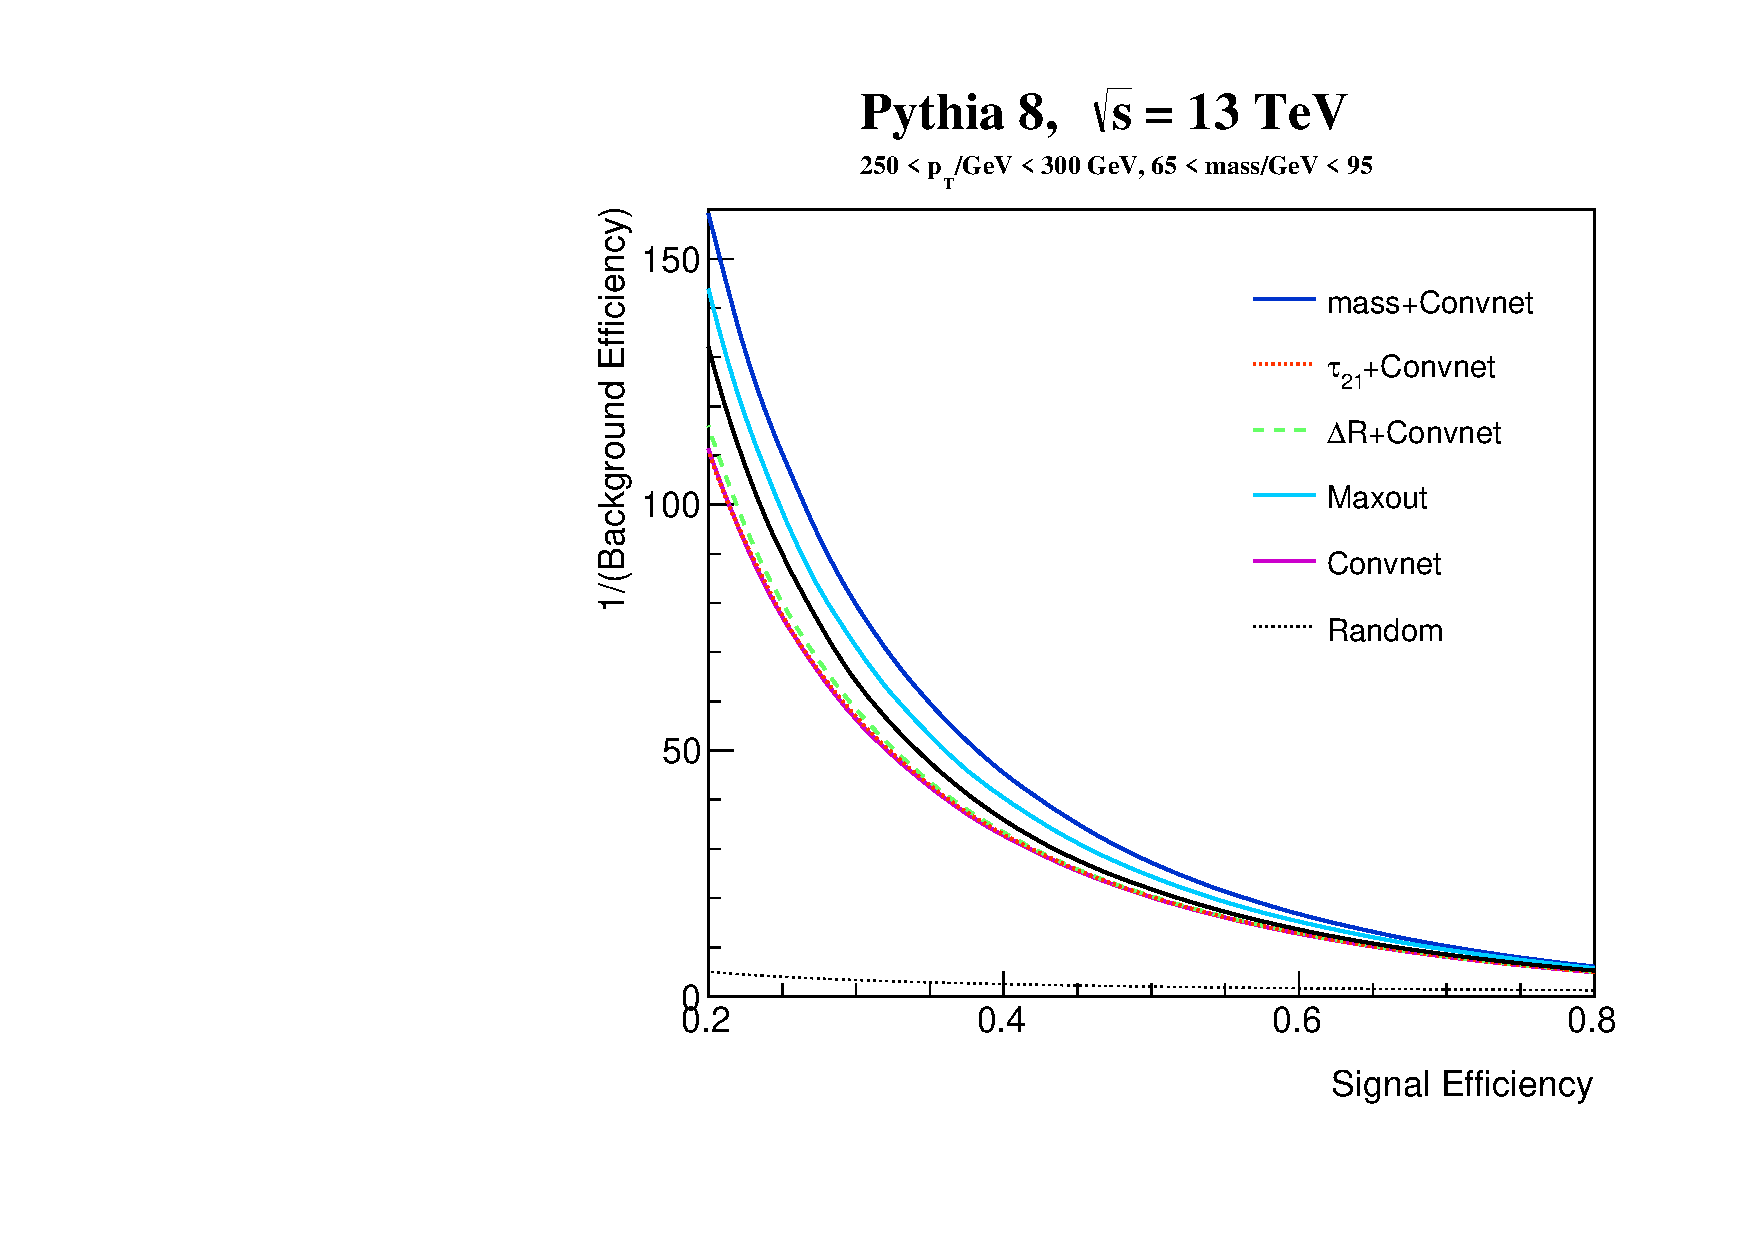
\includegraphics[width=0.48\textwidth,angle=0]{figures/ROC_3}
	\label{fig:combinedROC2a}
}
\subfloat[]{
	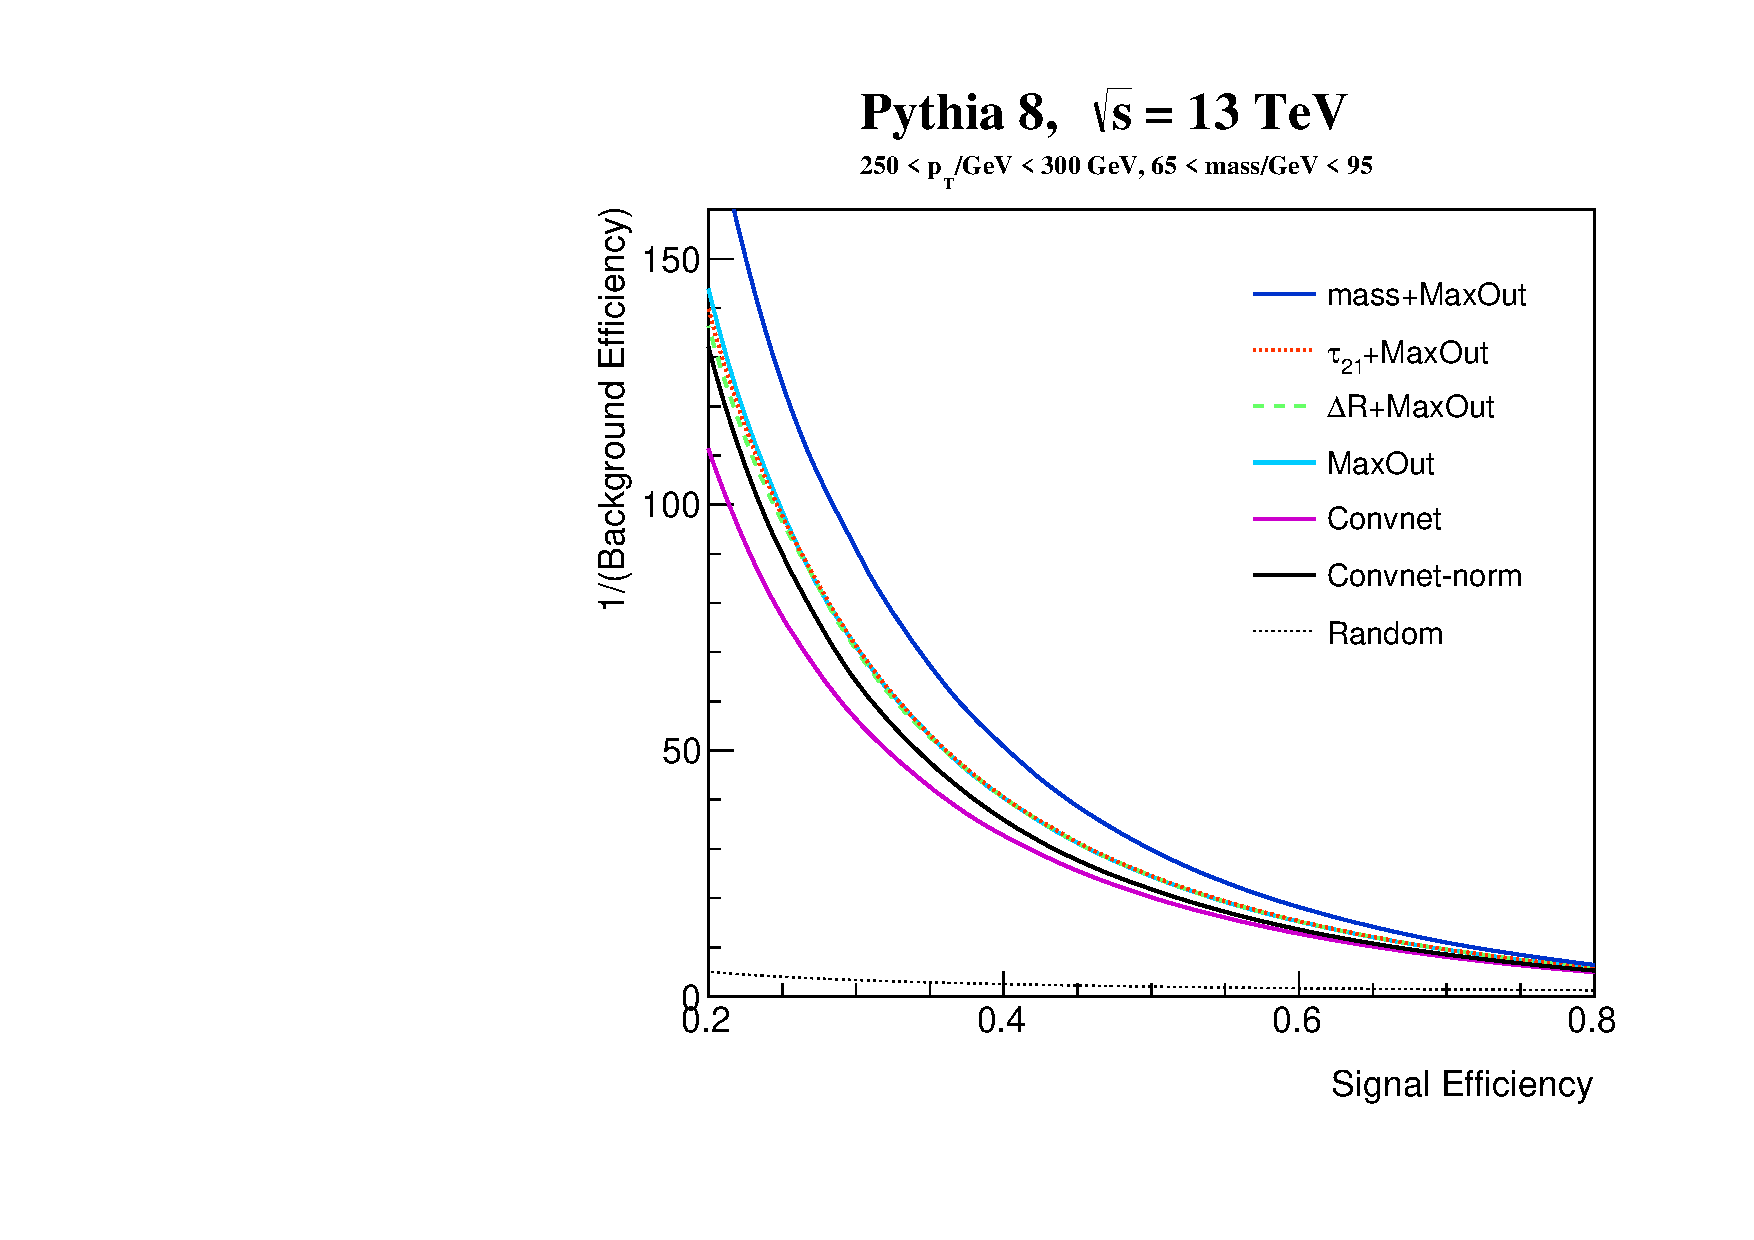
\includegraphics[width=0.48\textwidth,angle=0]{figures/ROC_4}
	\label{fig:combinedROC2b}
}
\end{center}
  \caption{Receiver Operating Characteristic (ROC) over coarse sample}
  \label{fig:combinedROC2}
\end{figure}

Another way to inspect what information about the physics-inspired variables has been learned by the DNN's is to study the correlation between the DNN output and the physics-variables.  The correlations are shown in Figure~\ref{fig:sculptedConv} for the ConvNet, and in Figure~\ref{fig:sculptedConv} for the MaxOut network,  against the jet mass, $\Delta R$, and $\tau_{21}$.   These distributions are normalized in bins of the DNN output, and thus the $z$-axis is showing the probability of the physics variable given the network output (i.e. $P($variable | network output$)$). Normalizing the distributions in this way allows us to see the most probable values of the physics variables at each point of the network output, without being affected by the overall distribution of jets in this 2D space.  We can see that both networks show a strong (non-linear) correlations with $\tau_{21}$ and $\Delta R$, giving further evidence that this information has been learned by the networks.  However, the correlations are much weaker with the jet mass variable, being slightly more strongly correlated with the MaxOut network output.  While it is not shown, similar patterns are found for the Conv-Norm network.
\begin{figure}[htbp!]
  \begin{center}
  
  \subfloat[Sculpted QCD  ConvNet network output versus mass (left), $\Delta R$ (middle), and $\tau_{21}$ (right) distributions\label{fig:sculptedConv}]
      {
        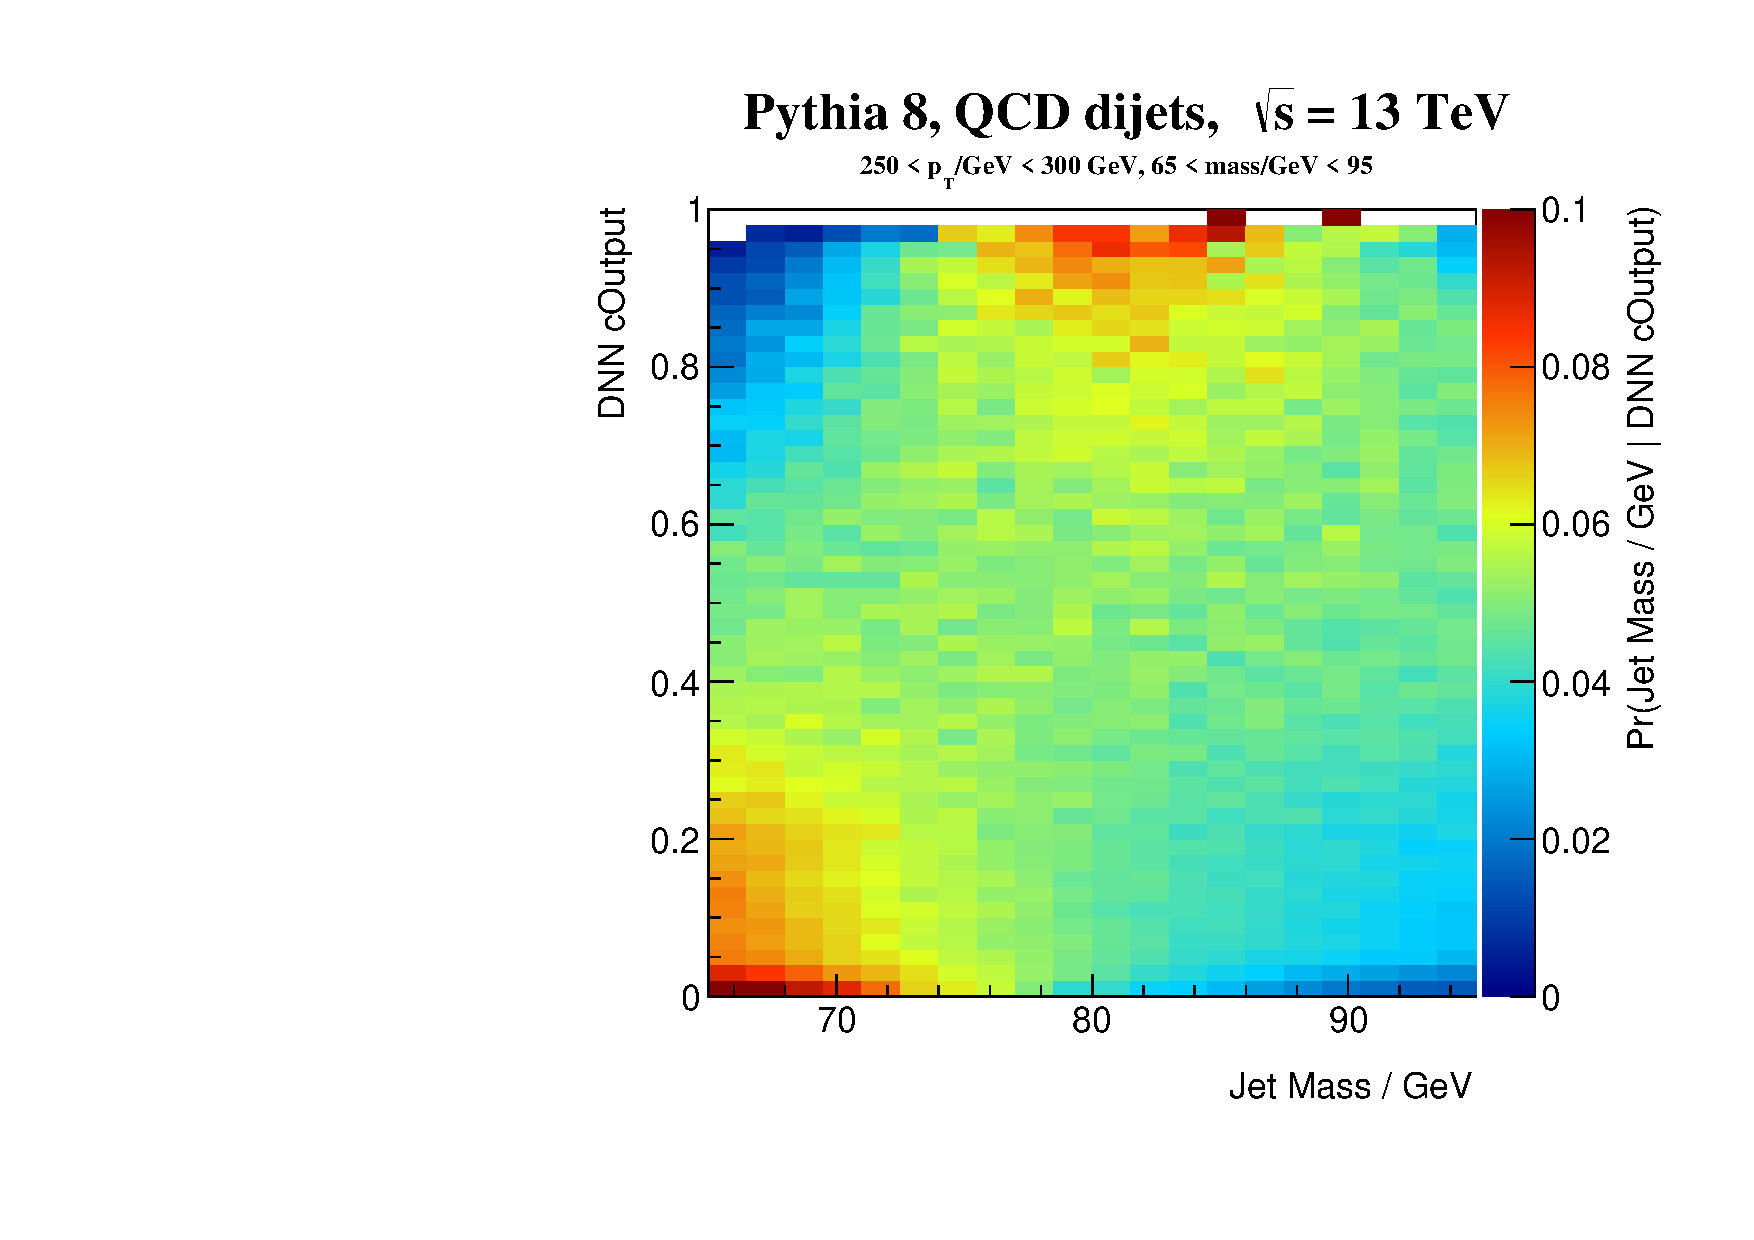
\includegraphics[width=0.32\textwidth]{figures/mass_convnet_back_norm_invert.pdf}
         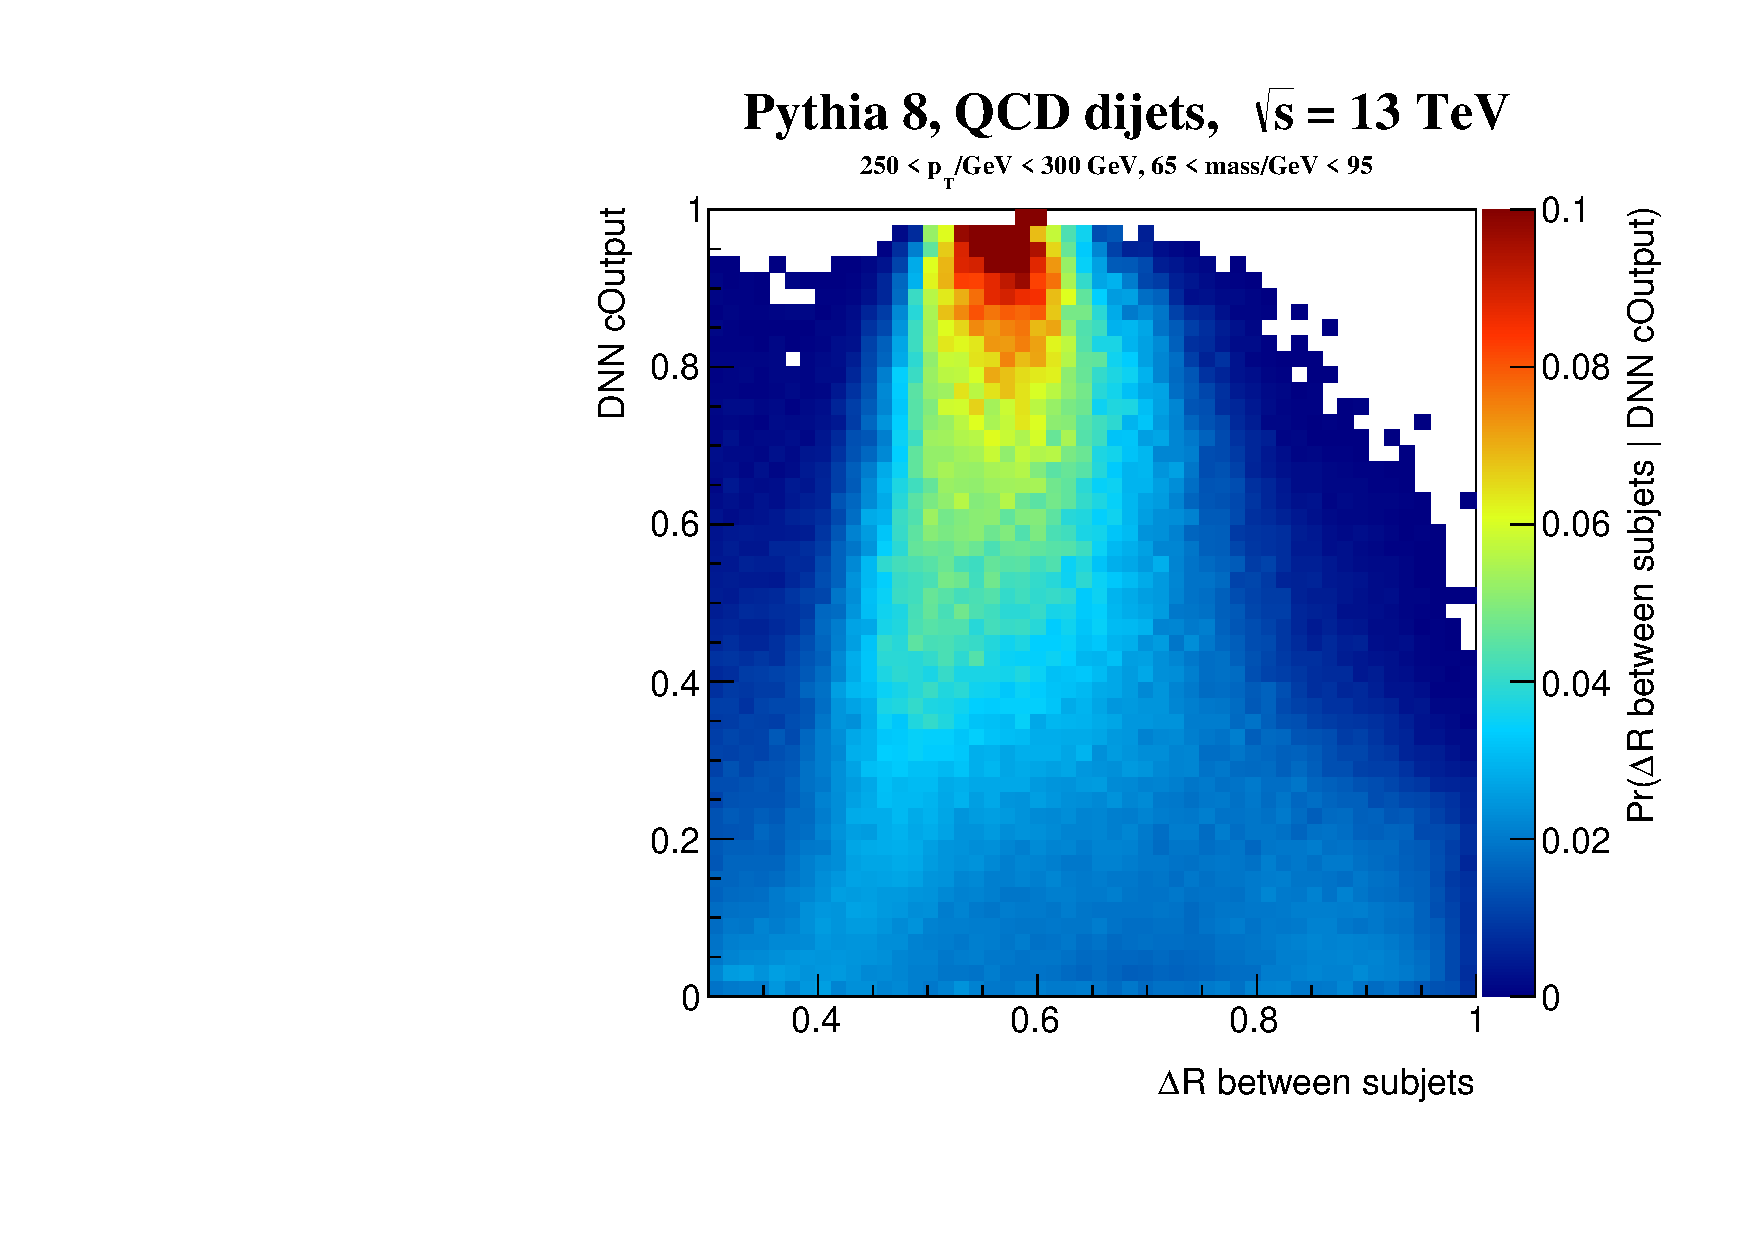
\includegraphics[width=0.32\textwidth]{figures/dR_convnet_back_norm_invert.pdf} 
         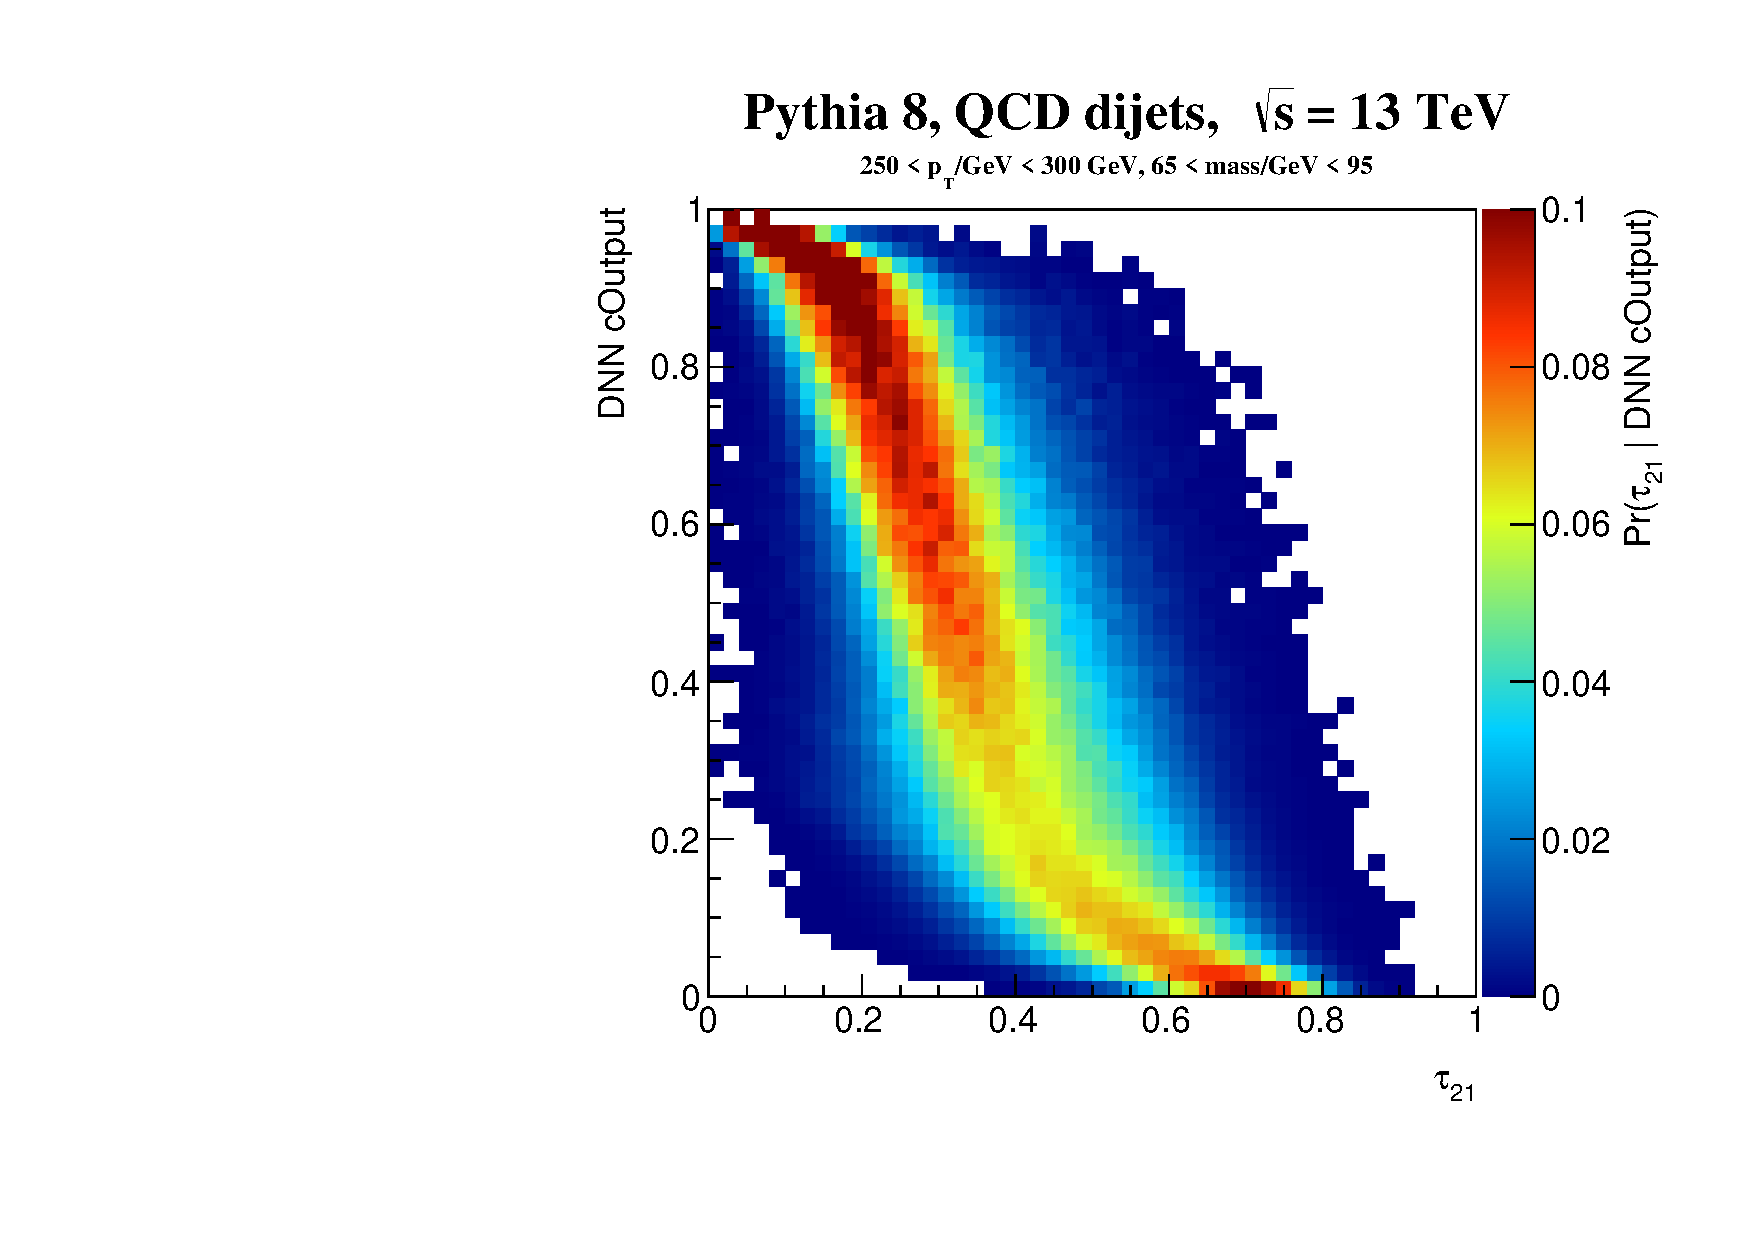
\includegraphics[width=0.32\textwidth]{figures/tau21_convnet_back_norm_invert.pdf}
      }\\
        \subfloat[Sculpted QCD  MaxOut network output versus mass (left), $\Delta R$ (middle), and $\tau_{21}$ (right) distributions\label{fig:sculptedMax}]
      {
        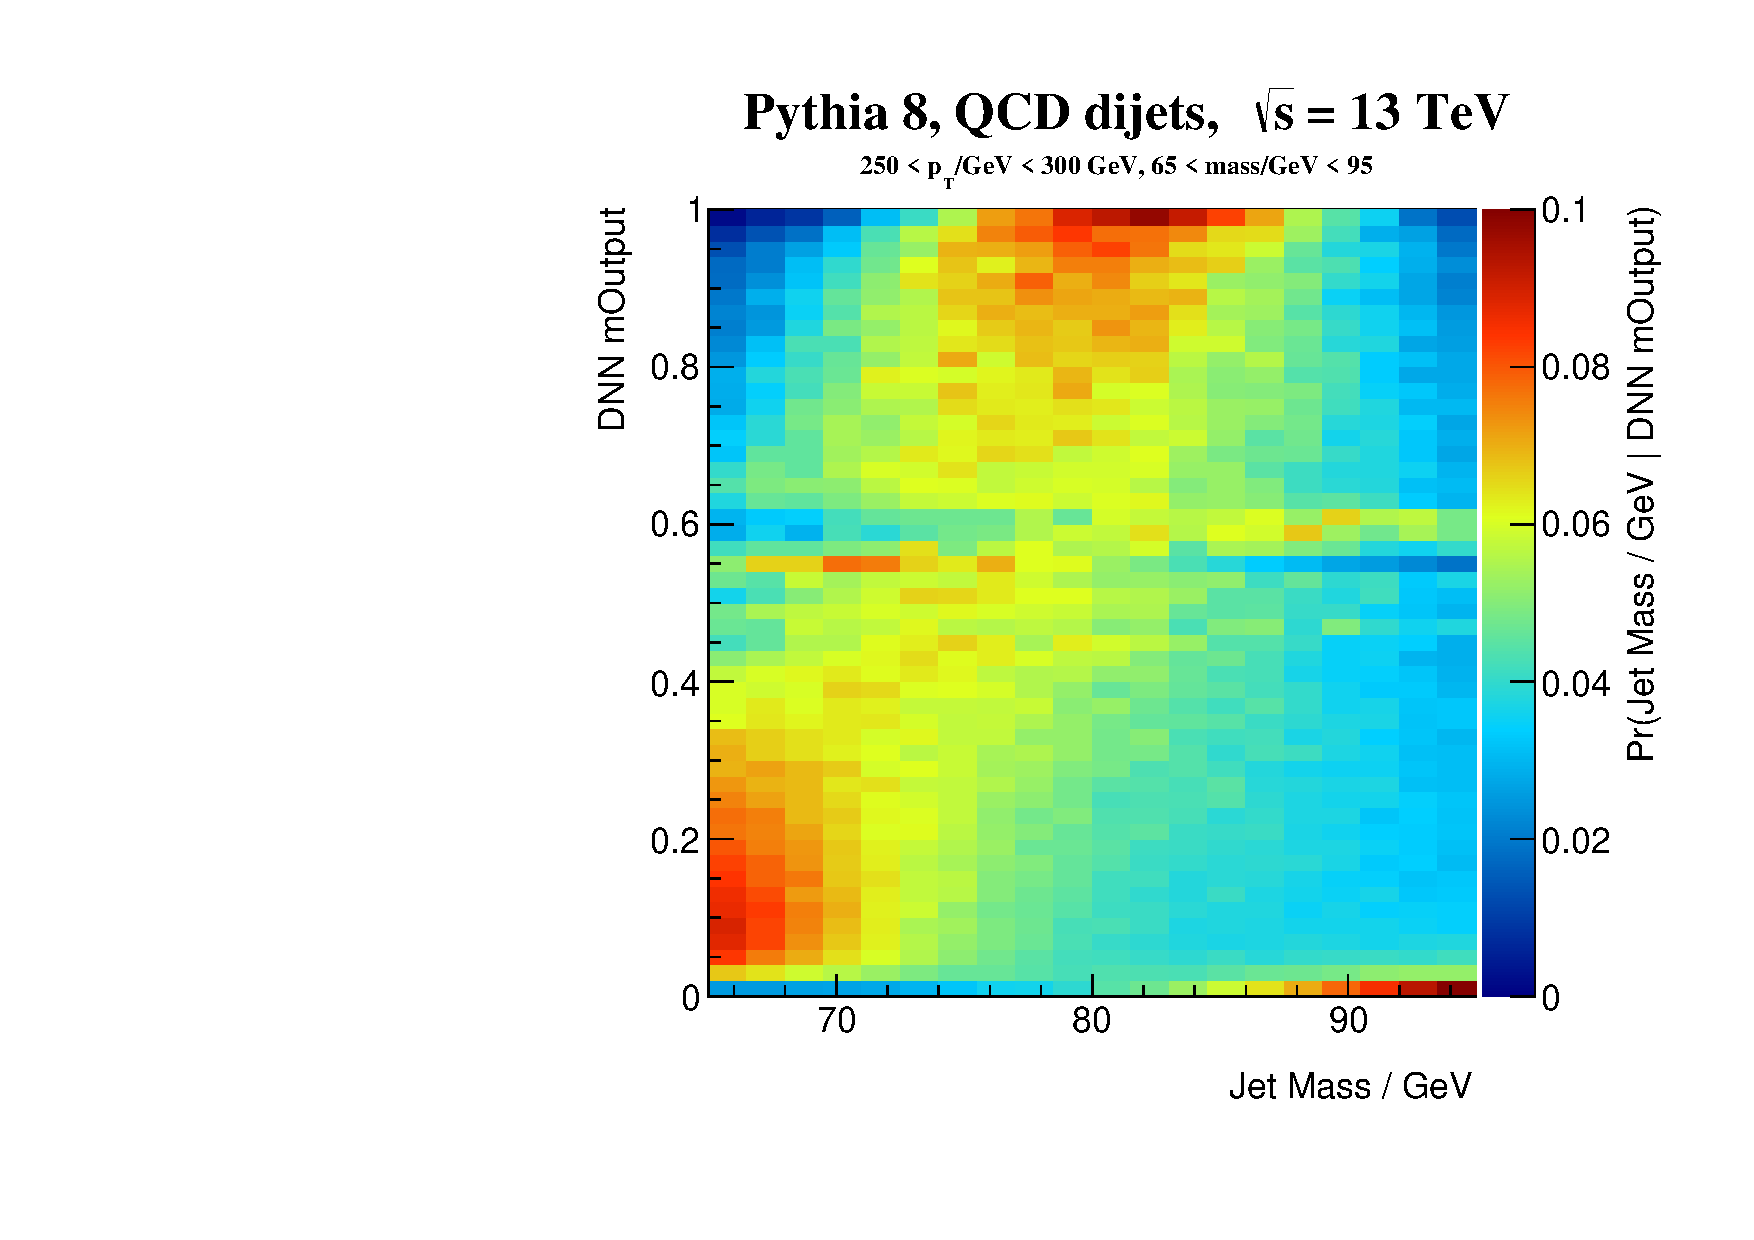
\includegraphics[width=0.32\textwidth]{figures/mass_maxout_back_norm_invert.pdf}
         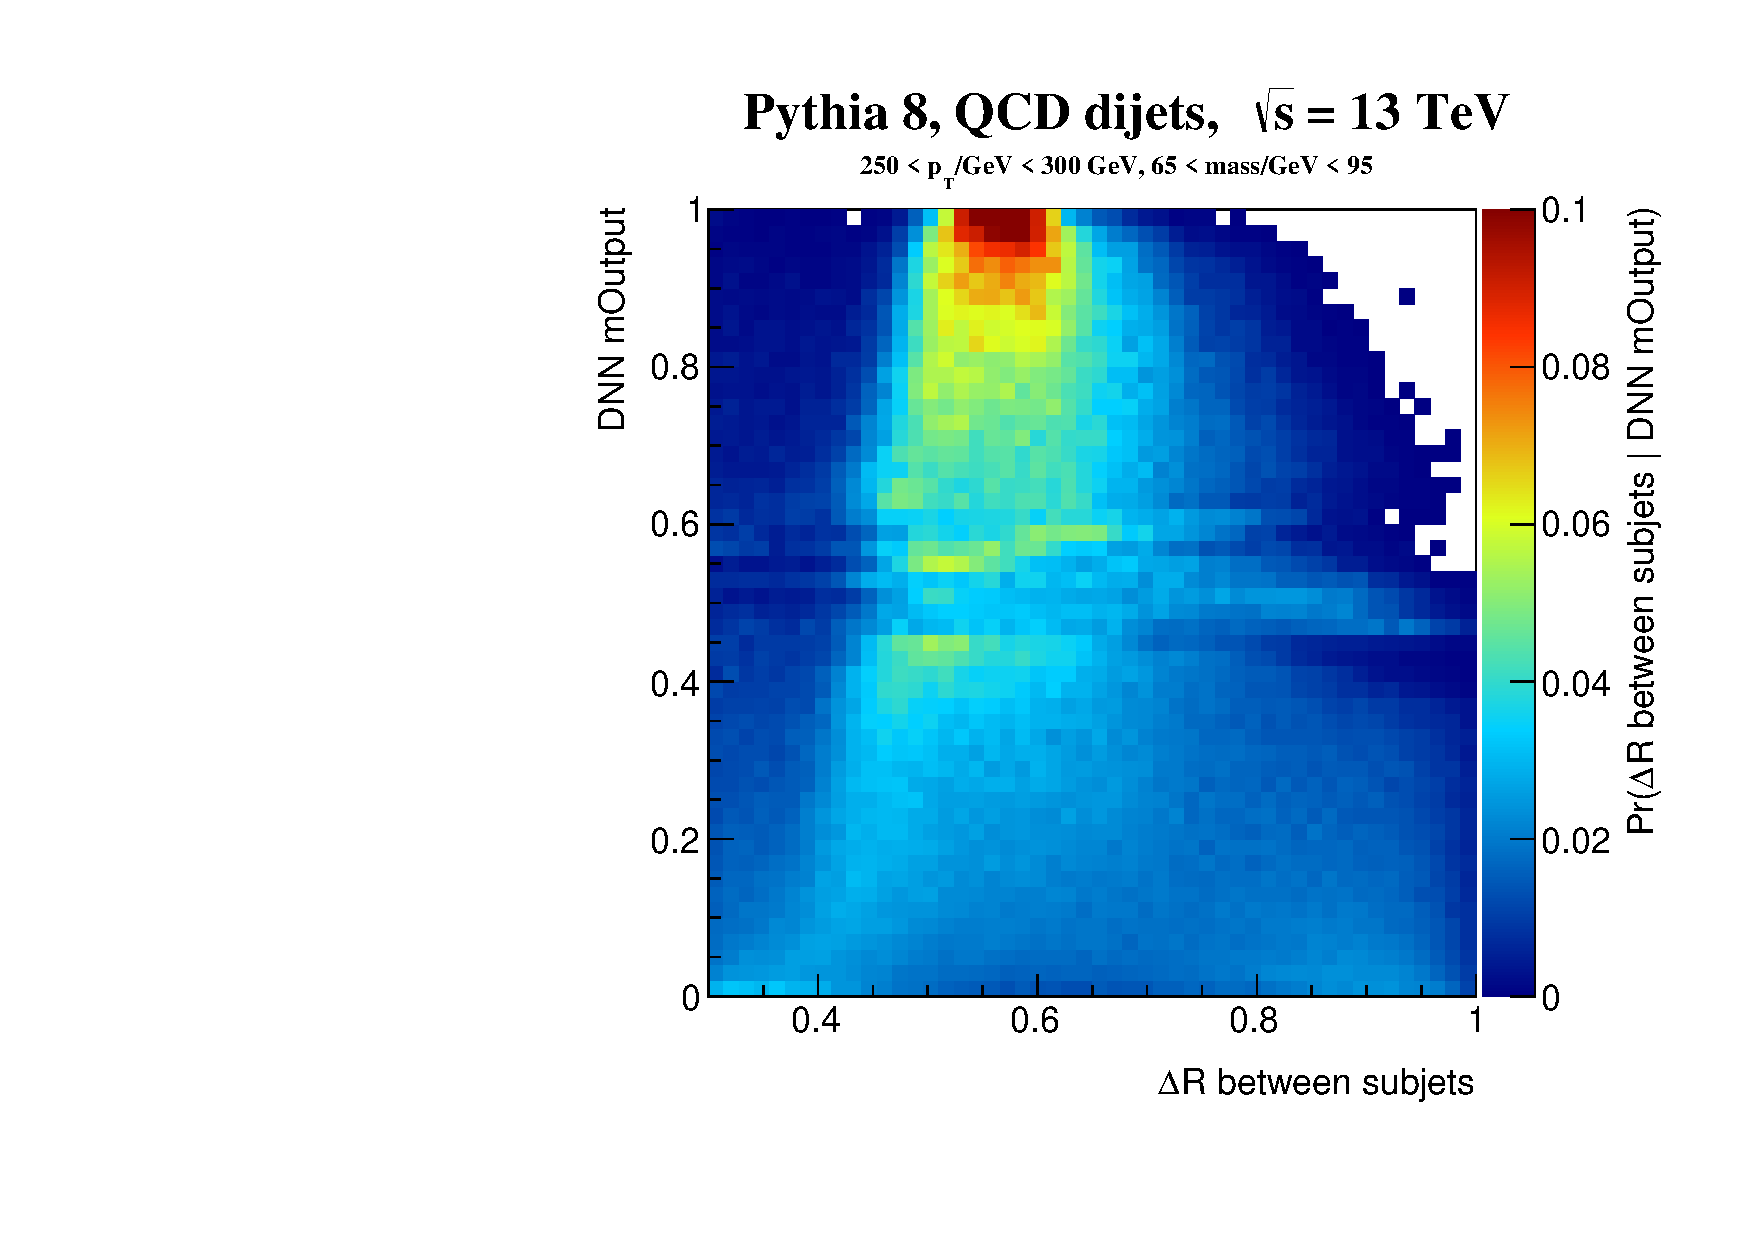
\includegraphics[width=0.32\textwidth]{figures/dR_maxout_back_norm_invert.pdf} 
         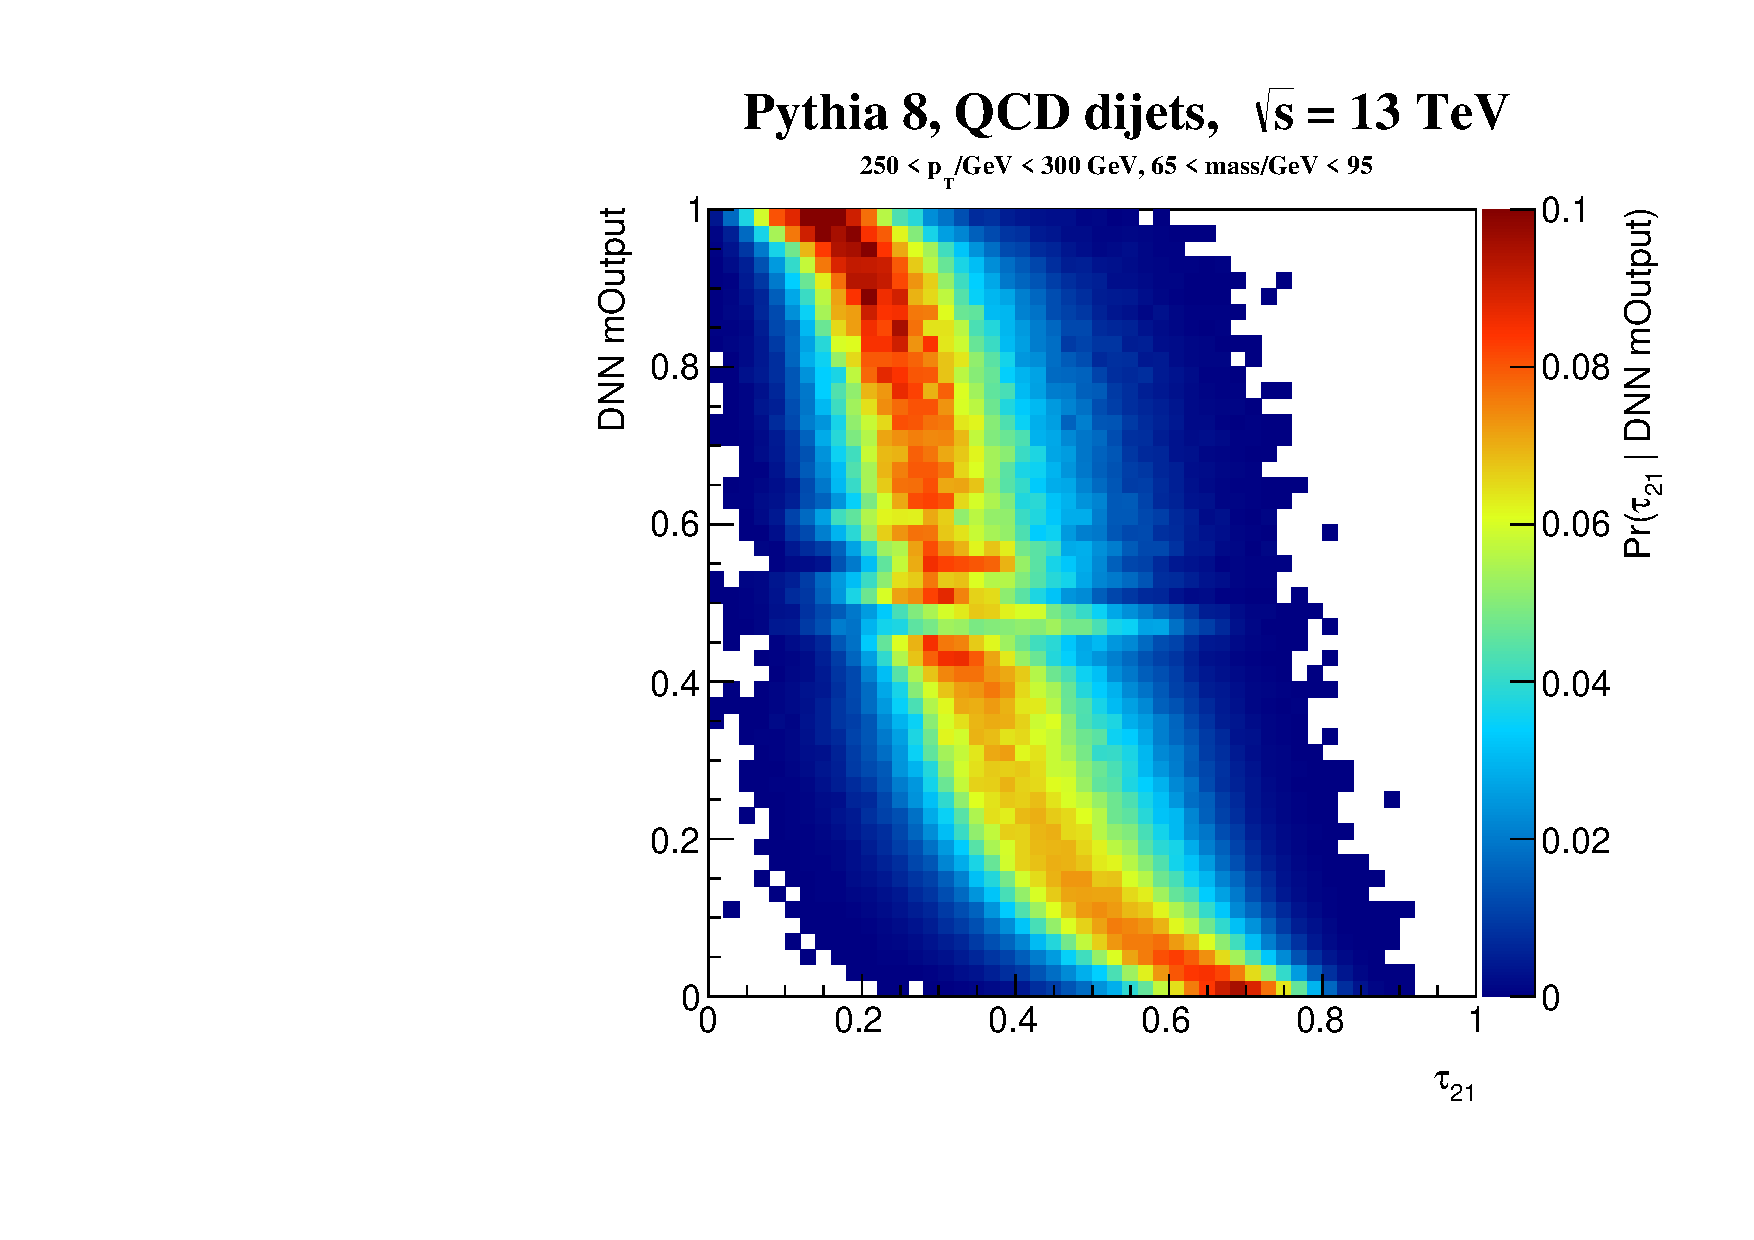
\includegraphics[width=0.32\textwidth]{figures/tau21_maxout_back_norm_invert.pdf}
      }\\

      \caption{Sculpted QCD distributions}
      \label{fig:qcdsculpt}

    \end{center}
\end{figure}

\subsubsection{Understanding what is learned} % (fold)
\label{ssub:understanding_what_is_learned}

Though important on it's own, the ROC curves only begin to help us understand what information has been learned. The increased performance of the DNN's over the physics inspired variables and their combinations begs further questions: what is this gain, and where does it come from? Why is the DNN able to pick up on this? In order to improve our understanding of what we learn, we first take a look \emph{inside} the deep network, and visualize features learned during training.


In Figure~\ref{subfig:filters}, we show the first layer 11$\times$11 convolutional filters learned by our Conv-Norm network. Each filter is visualized by showing the learned weight in each position of the filter.  We can see that there is variation between filters, indicating that they are learning different features of the jet-images, but this variation is not as large as seen in many CV problems due to the sparsity of the jet-images.  We also see that they tend to learn representations of the subjets and distances between subjets, as seen by the circular features found in many of the filters.

To get a better understanding of how these filters provide discrimination, we mimic the operation in the first layer of the network by convolving each filter with average of large samples of signal and background jet images.  The difference between the average signal and average convolved background jet-images help to provide an understanding of what difference in features the network learns at the first layer in order to help discriminate.

More formally, let $J_s=\frac{1}{n}\sum_{i:i\text{ is signal}} J^{(i)}$ and $J_b=\frac{1}{n}\sum_{i:i\text{ is background}}J^{(i)}$ represent the average signal and background jet over a sample, where $J^{(i)}$ is the $i$th jet image. In addition, we can select a filter $w_i\in\mathbb{R}^{11\times11}$ from the first convolutional layer. We then examine the differences in the post convolution layer by computing:
\begin{equation}
  J_s \ast w_i - J_b \ast w_i, \forall i,
\end{equation}

where $\ast$ is the convolution operator. We arrange these new ``convolved jet-images'' in a grid, and show in red regions where signal has a stronger representation, and in blue where background has a stronger representation. In Figure~\ref{subfig:convolvedfilters}, we show the convolved differences described above, where each $(i, j)$ image is the representation under the $(i, j)$ convolutional filter. We note the existence of interesting patterns around the regions where the leading and subleading subjets are expected to be. We also draw attention to the fact that there is a large diversity in the the convolved representations, indicating that the DNN is able to learn and pick up on multiple features that are descriptive.
\begin{figure}[bt]
  \begin{center}
      \subfloat[$(11\times11)$ convolutional kernels from first layer \label{subfig:filters}]{
        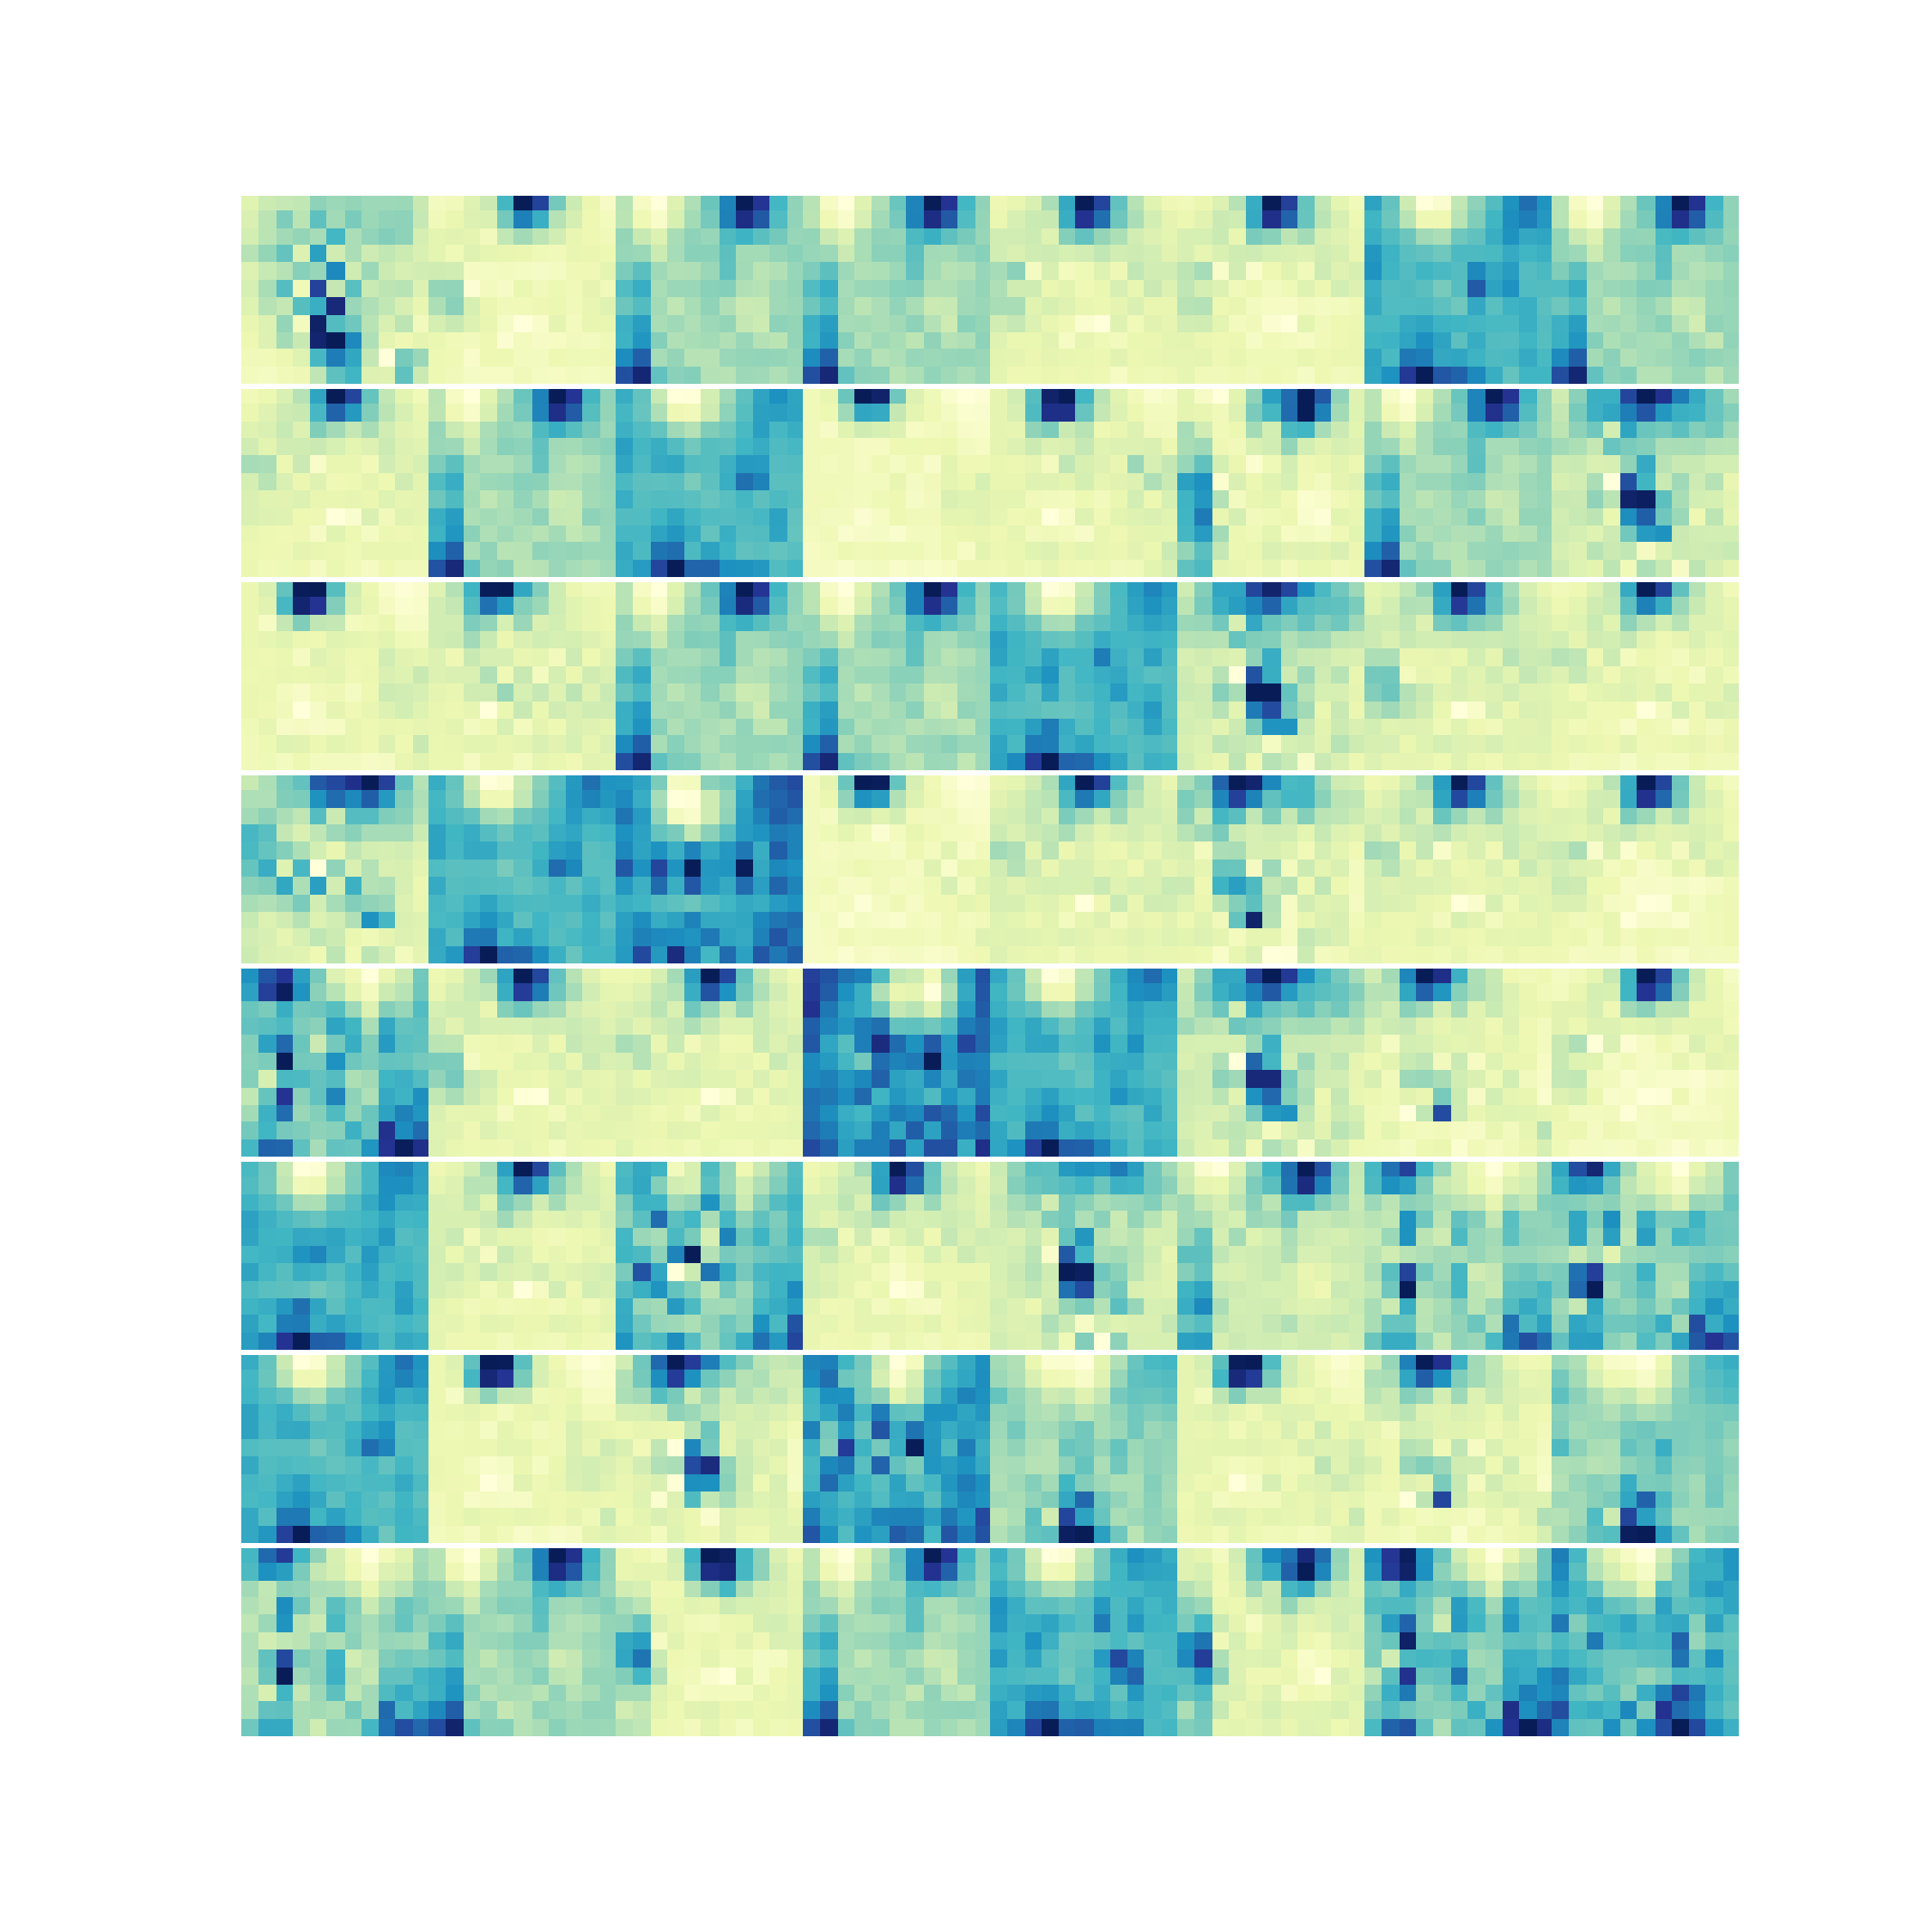
\includegraphics[width=0.5\textwidth]{figures/conv-filts.pdf}
      }
      \subfloat[Convolved Jet Image differences\label{subfig:convolvedfilters}]{
        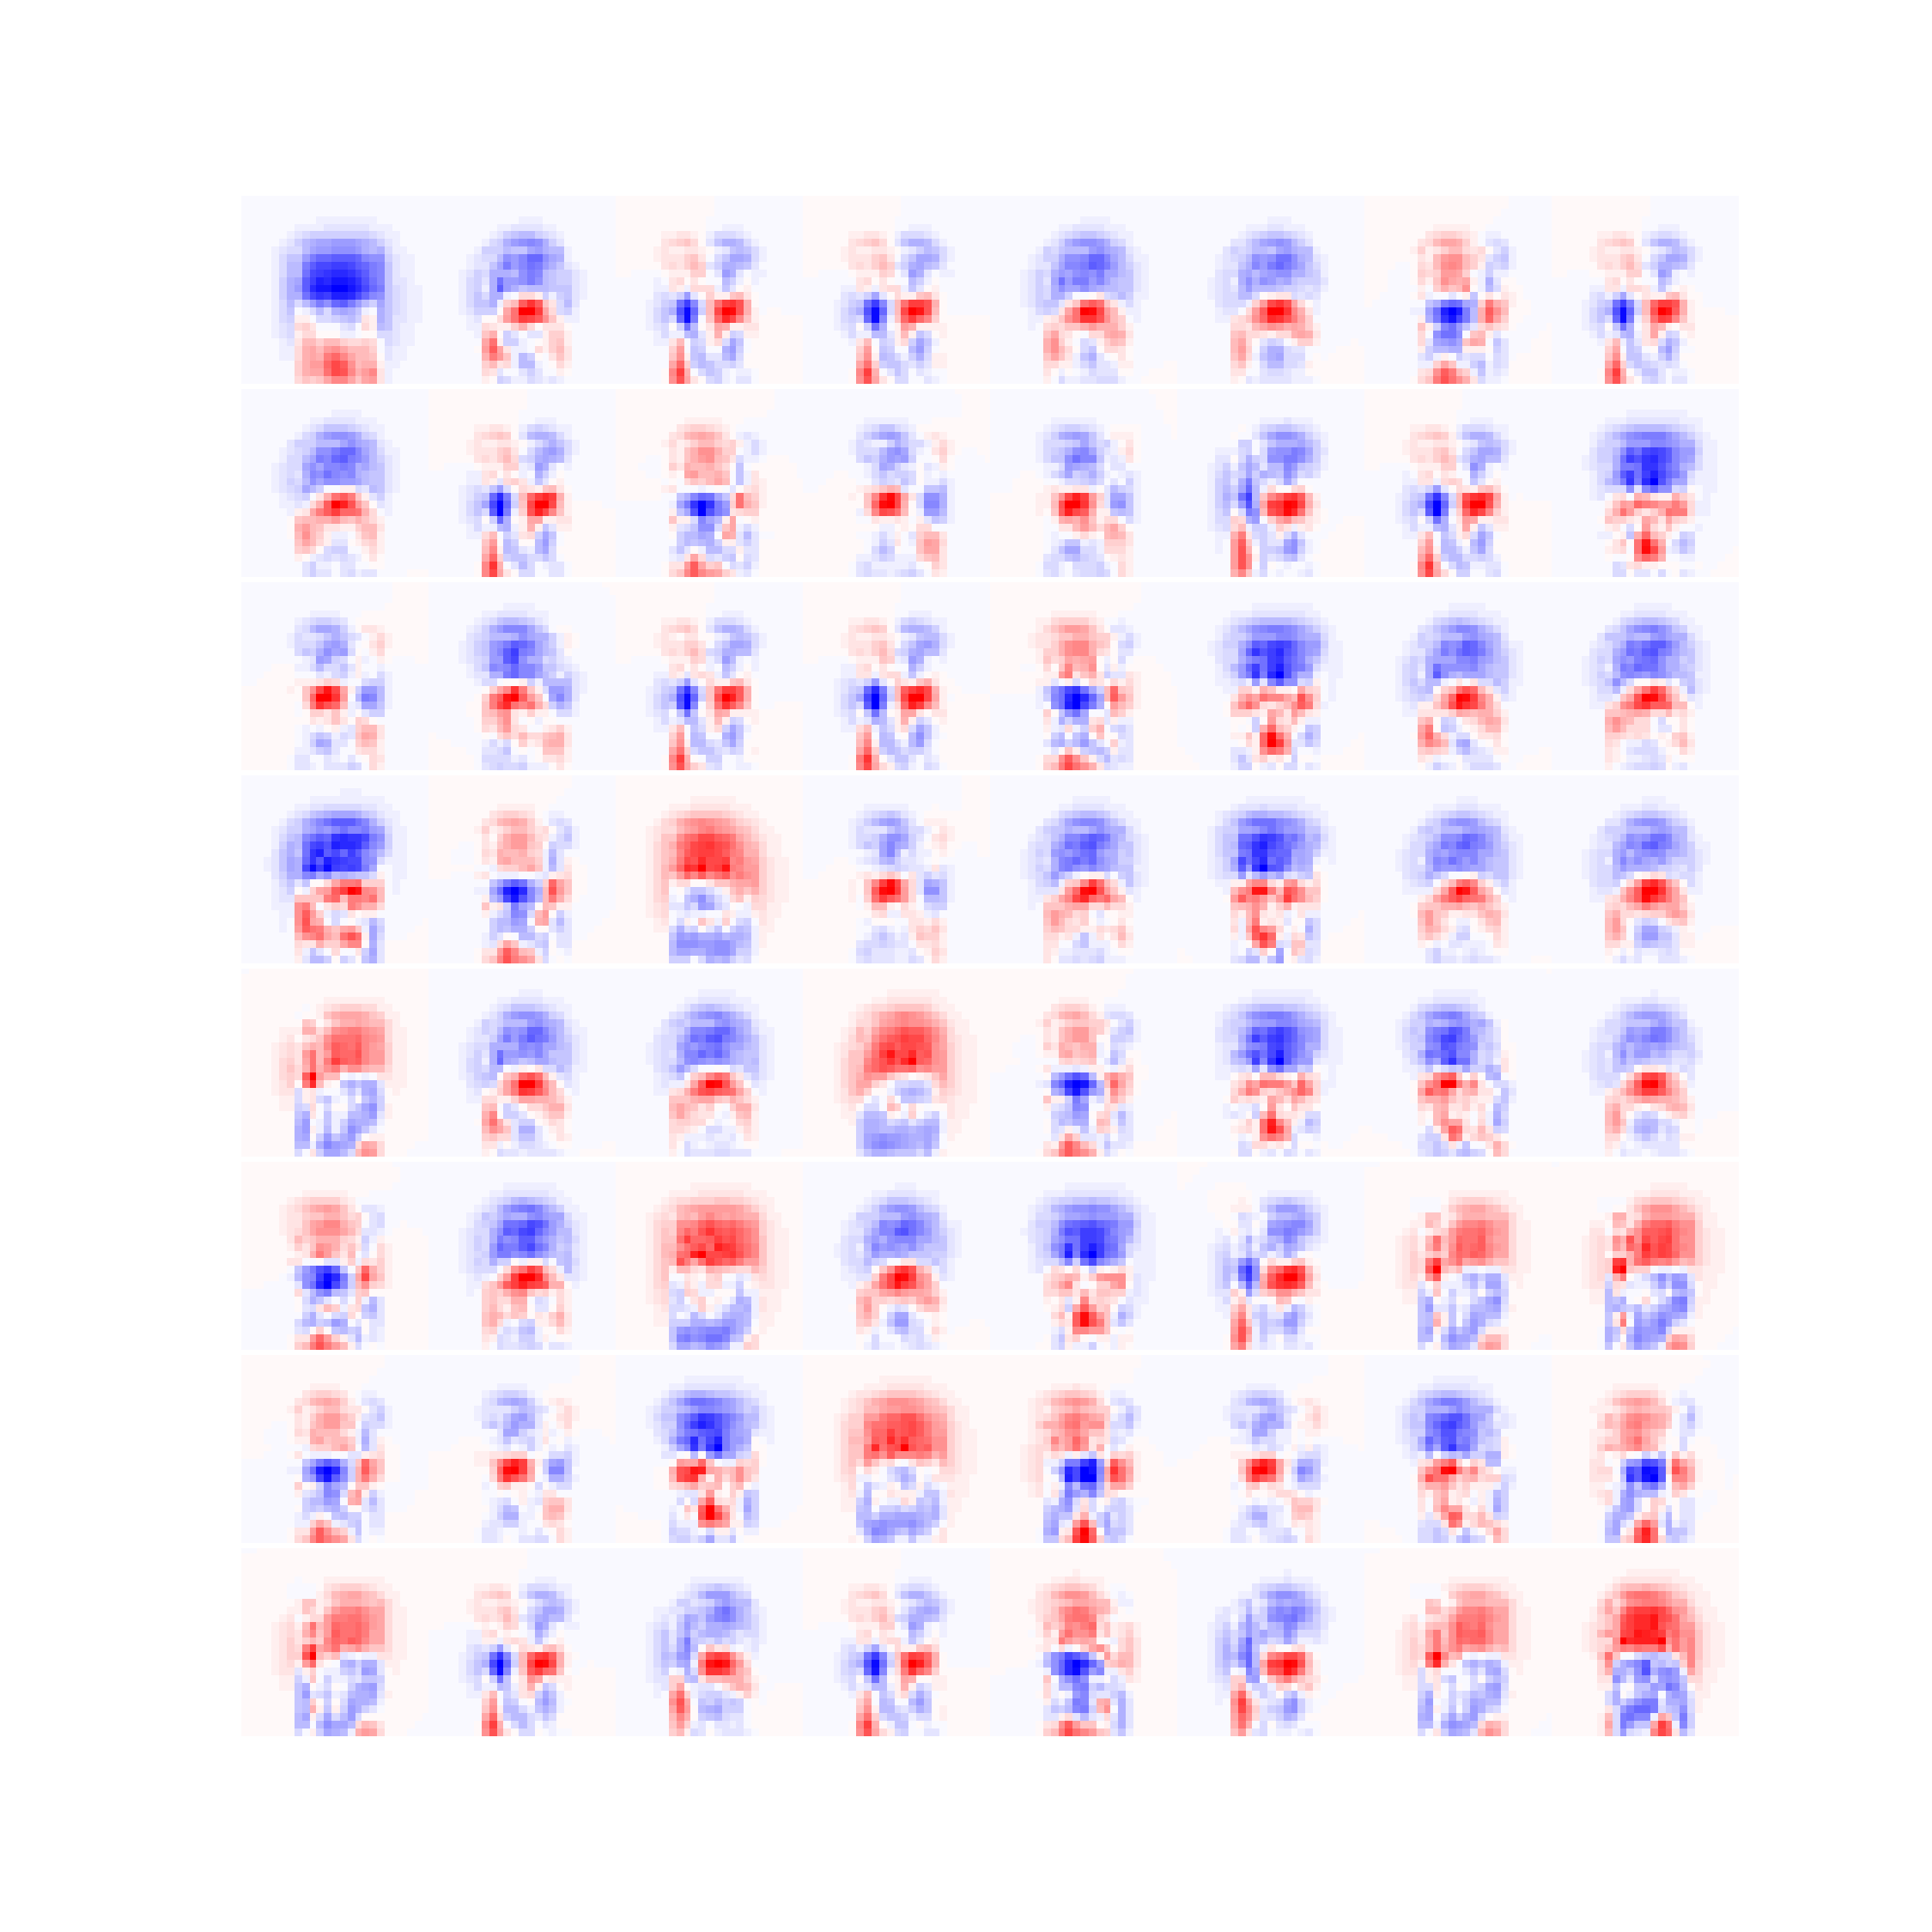
\includegraphics[width=0.5\textwidth]{figures/conv-diffs-global.pdf}
      }
      \caption{Convolutional Kernels (left), and convolved feature differences in jet images (right)}
      \label{fig:convkernels}

    \end{center}
\end{figure}


For every node in the last hidden layer in the maxout network (i.e., the layer before the classification layer) we examine the node activations, and take the weighted (by pT flat  weights) average of the top 501 jet images that activate that node. Then, we order the nodes from top left to bottom right by increasing sparsity -- that is, we go from least sparse (most commonly activated and > 0) to most sparse (least commonly activated and frequently equal to zero). Fig.~\ref{fig:mostactiviate}.

\begin{figure}[!htbp]
  \centering
  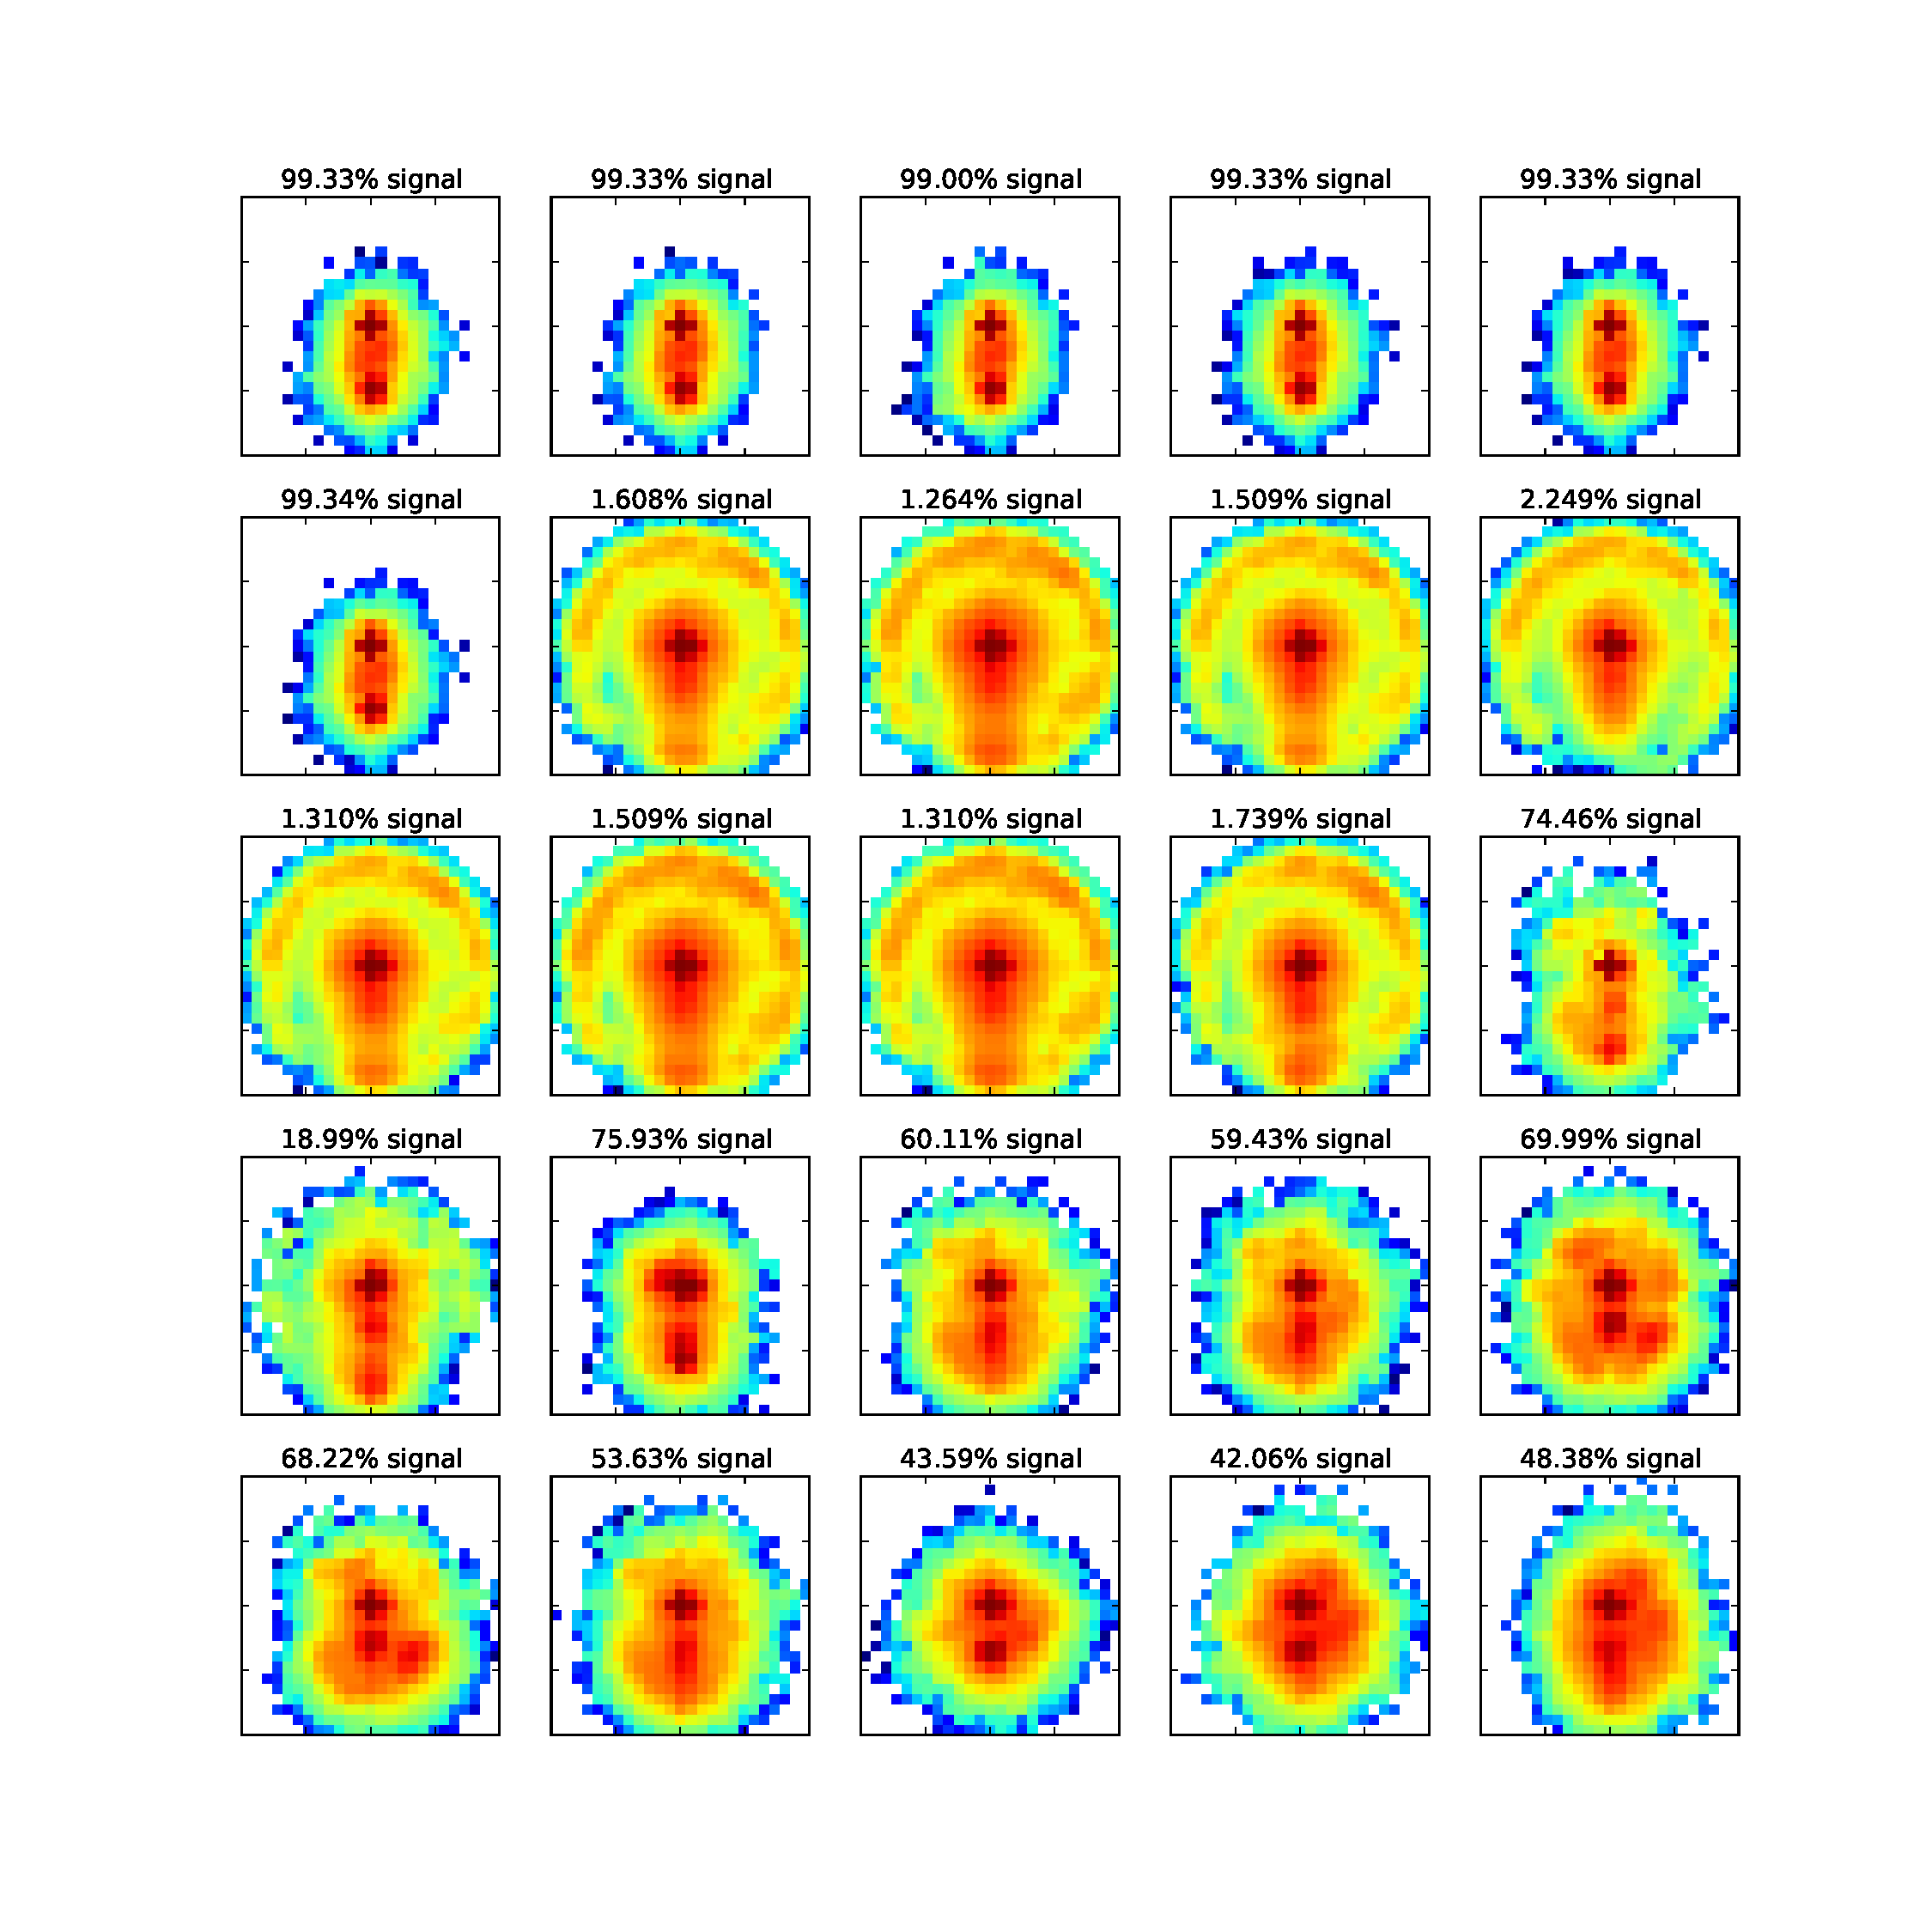
\includegraphics[width=0.8\textwidth]{figures/maxnodes.pdf}
  \caption{caption.}
  \label{fig:mostactiviate}
\end{figure}




\subsubsection{Physics in Deep Representations} % (fold)
\label{ssub:physics_in_deep_representations}
To get a tangible and more intuitive understanding of what jet structures a DNN learns, we compute the correlation of the Conv-Norm network output with each pixel of the jet-images. Specifically, let $y$ be the DNN output, and consider every pixel $p_ij$ in transformed $(\eta, \phi)$ space. We the construct an image, which we denote the \emph{deep correlation jet-image}, where each pixel $(i, j)$ is $\rho_{p_{ij}, y}$, the Pearson Correlation Coefficient of that pixels energy deposition with the final DNN output. While this this image does not give a direct view of the discriminating information learned within the network, it does provide a guide to how such information may be contained within the network.  In Figure~\ref{fig:corr}, we construct this deep correlation jet-image, and can see a wealth of interesting structure.  We can see that the location and energy of the subleading subjet, found at the bottom of the image, is highly correlated with the DNN output and important for identifying signal jet-images.  In contrast, the information contained in the leading subjet, seen at $(x,y)\sim (0,0)$ in the image, is not particularly correlated with the network owing to the fact that both signal and background jets have high energy leading subjets.  We also see asymmetric regions around both subjets that are correlated with the DNN output and is likely indicating the presence of additional radiation expected in the QCD background jets.  Finally, a small negative correlation with the rest of the jet area is seen, indicating that radiation from the background jets is more likely to be observed in these regions.   The exact function form of this distribution is not known, nor does it seem to describe exactly any known physics inspired variable.
\begin{figure}[!htbp]
  \centering
  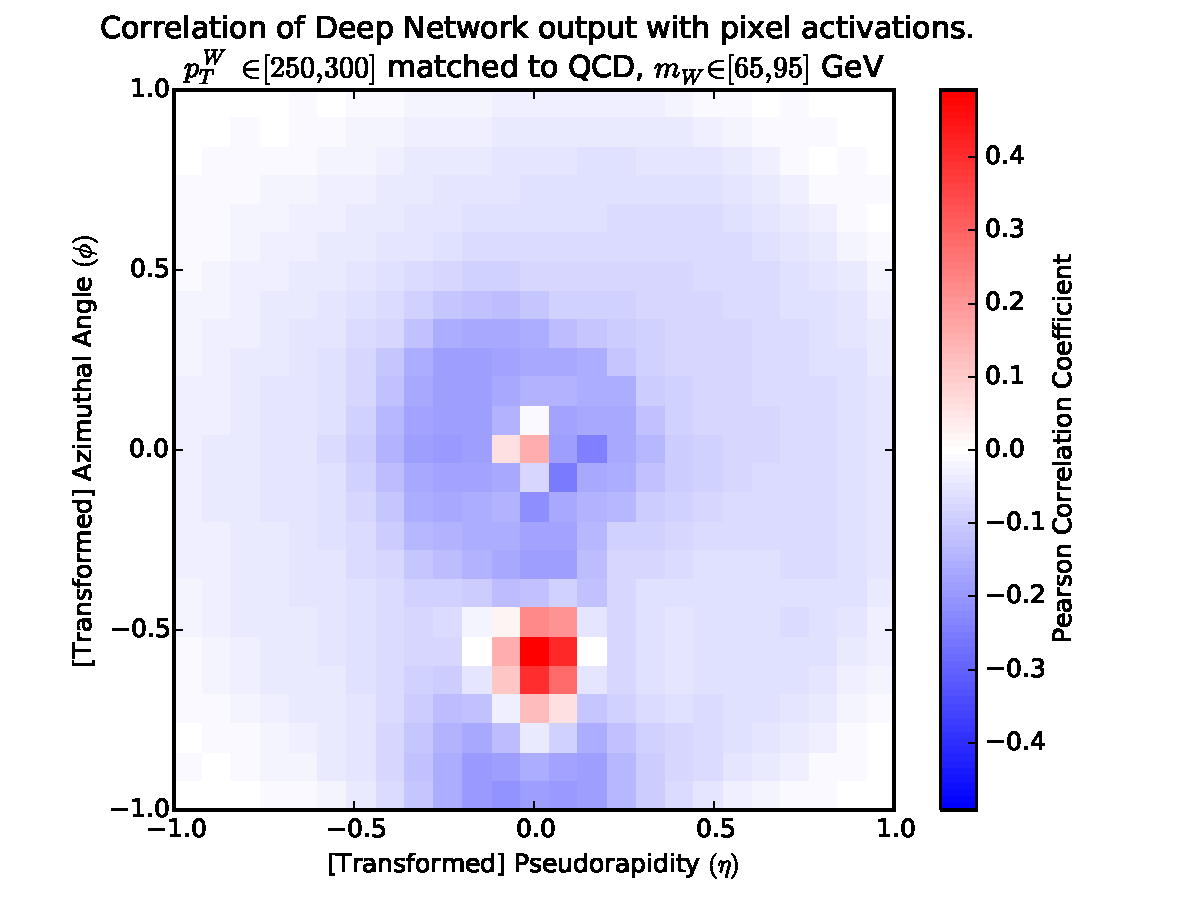
\includegraphics[width=0.5\textwidth]{figures/pixel-activations-corr.pdf}
  \caption{Per-pixel linear correlation with DNN output}
  \label{fig:corr}
\end{figure}

